Die Systemtheorie beschreibt Systeme unter anderem durch den Zusammenhang von Signalen am Systemeingang und Systemausgang. In Teil A dieser Buchreihe sind Beispiele für unter-schiedliche zeitkontinuierliche Signalformen dargestellt. Außerdem sind dort bereits Eigenschaf-ten und Rechenregeln für zeitkontinuierliche Signale beschrieben. In diesem Kapitel werden zeitdiskrete Signale behandelt. \medskip

\noindent Im ersten Abschnitt wird die Klassifizierung von zeitkontinuierlichen Signalen auf zeitdiskrete Signalfolgen übertragen. \medskip

\noindent Für die Charakterisierung von zeitdiskreten Systemen können Testfolgen als Eingangssignal ein-gesetzt werden, die eine besonders anschauliche Interpretation des Ausgangssignals ermöglichen. Bei zeitdiskreten Systemen ist dabei die Impulsfolge von großer Bedeutung, weil sie sich als reale Signalfolge darstellen lässt und eine anschauliche Interpretation der Systemantwort ermög-licht. Die Impulsfolge und ähnliche Folgen werden im zweiten Teil dieses Kapitels diskutiert und das Rechnen mit diesen Testfolgen an Beispielen erläutert.\medskip

\noindent Auch für zeitdiskrete LTI-Systeme gilt das Superpositionsprinzip. Kann ein Eingangssignal aus einer Linearkombination bekannter Signalfolgen beschrieben werden, ergibt sich das Ausgangs-signal aus derselben Linearkombination der zugehörigen Ausgangssignale. Deshalb wird im drit-ten Teil dieses Kapitels das Rechnen mit Signalfolgen vorgestellt.\medskip

\noindent Die Reaktion eines zeitdiskreten Systems kann vielfach über Kosinus- und Exponentialfolgen beschrieben werden. Beide Folgen können zu komplexen Exponentialfolgen zusammengefasst werden. Komplexe Exponentialfolgen werden dazu verwendet, das Einschwingverhalten von Systemen effizient zu beschreiben. Der vierte Teil dieses Kapitels widmet sich daher harmoni-schen Schwingungsfolgen sowie reellen und komplexen Exponentialfolgen.\medskip

\noindent Die hier dargestellten Signaleigenschaften und Rechenmethoden sind denen im zeitkontinuierli-chen Bereich sehr ähnlich. Sie sind hier trotzdem ausführlich aufgeführt, um einen Quereinstieg in das Thema der zeitdiskreten Systeme zu ermöglichen.

\subsection{Klassen und Eigenschaften von Signalen}

\noindent In Teil A dieser Buchreihe werden verschiedene Signalklassen dargestellt. Die dort vorgestellten Signalklassen und Eigenschaften beziehen sich auf zeitkontinuierliche Signale. Mit der Abtas-tung von Signalen werden Signale zeitquantisiert. Wie bereits in Kapitel \ref{two} dargestellt wird, wird bei der Beschreibung der abgetasteten Signale die Amplituden-Quantisierung gerne vernachläs-sigt, sodass im vorliegenden Teil B dieser Buchreihe zeitdiskrete Systeme mit kontinuierlicher Amplitude behandelt werden. Diese Signale sind in Bild \ref{fig:DiskreKontinuerlich} oben rechts dargestellt.
\clearpage
\begin{figure}[H]
  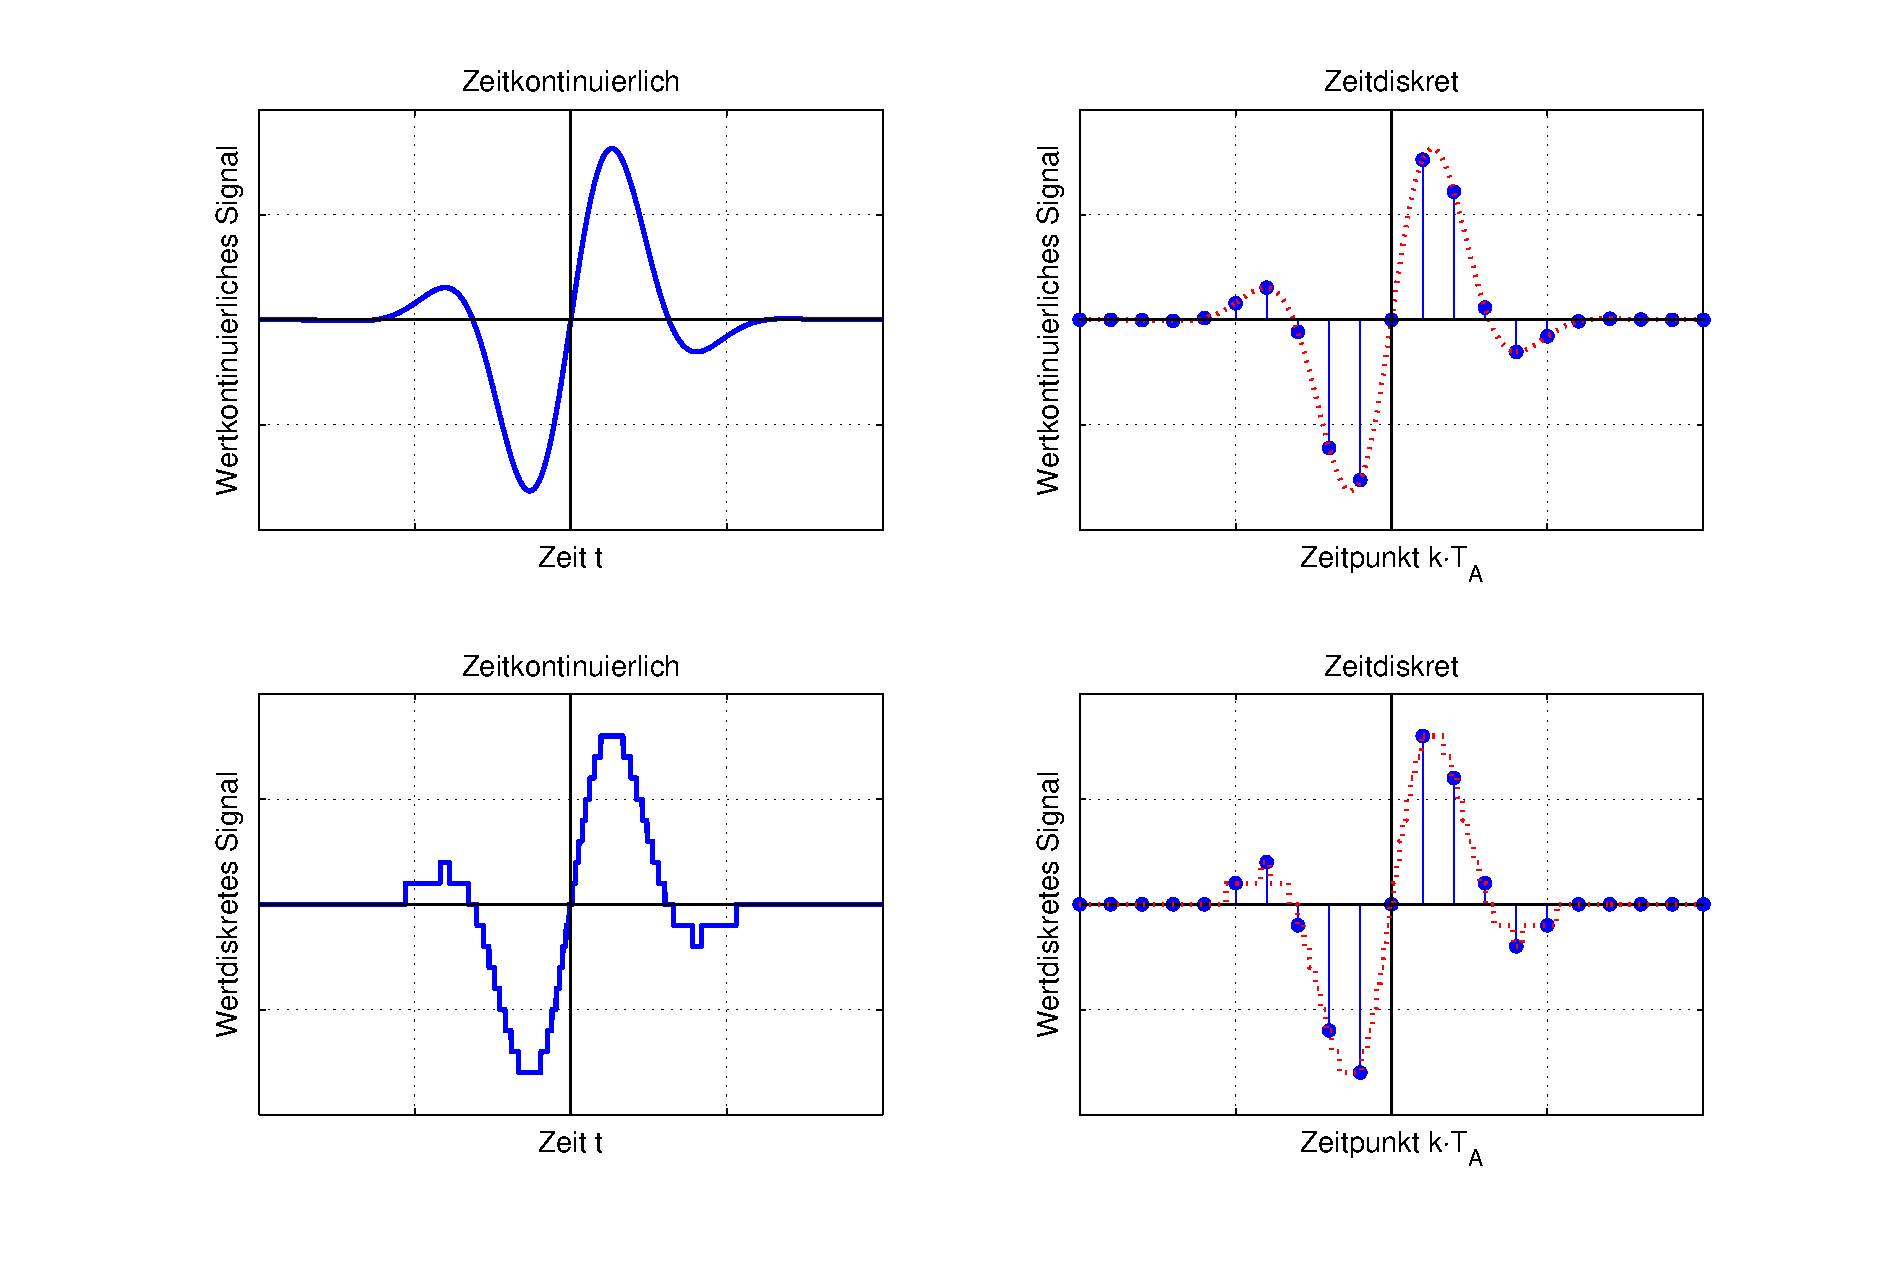
\includegraphics[width=1.0\textwidth]{Kapitel3/Bilder/image1.eps}
  \caption{Darstellung wertkontinuierlicher und wertdiskreter Signale in zeitkontinuierlicher und zeitdiskreter Form}
  \label{fig:DiskreKontinuerlich}
\end{figure}

\noindent Zeitdiskrete Signale sind nur zu bestimmten Zeitpunkten definiert. Es existieren keine Übergänge zwischen zwei aufeinanderfolgenden Werten. Im Fall der Abtastung eines zeitkontinuierlichen Signals x(t) ergibt sich die Zahlenfolge x[k] des abgetasteten Signals zu

\begin{equation}\label{eq:threeone}
x\left[k\right]=x\left(k\cdot T_{A} \right)
\end{equation}

\noindent Da die Signale nicht mehr kontinuierlich sind, werden sie als Folgen oder Signalfolgen x[k] bezeichnet. Mit den eckigen Klammern wird der Unterschied zwischen zeitkontinuierlichen Signa-len x(t) und Signalfolgen x[k] grafisch verdeutlich. Bild \ref{fig:Signalfolge} zeigt ein Beispiel für eine Signalfolge.

\begin{figure}[H]
  \centerline{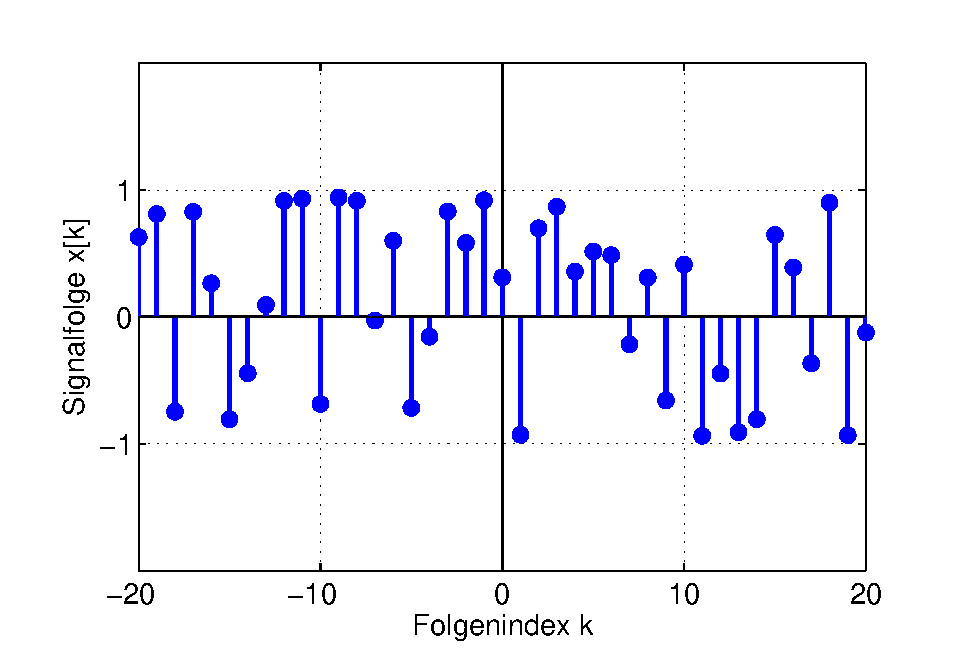
\includegraphics[width=0.5\textwidth]{Kapitel3/Bilder/image2.eps}}
  \caption{Darstellung einer Signalfolge x[k]}
  \label{fig:Signalfolge}
\end{figure}

\noindent Da die Signalfolge x[k] nur zu definierten Zeitpunkten k$\cdot$T$_{A}$ definiert ist, können mathematische Operationen wie Integral und Differential nicht ausgeführt werden. Sie müssen durch entsprechende Operationen für Folgen ersetzt werden. Im ersten Abschnitt dieses Kapitels werden die wesentlichen bisher für zeitkontinuierliche Signale beschriebenen Signaleigenschaften und Re-chenoperationen auf zeitdiskrete Signale übertragen.

\subsubsection{Determinierte und zufällige Signalfolgen}

\noindent Determinierte Signalfolgen lassen sich durch eine mathematische Vorschrift in ihrem zeitlichen Verlauf angeben. Sie können implizit oder explizit definiert sein. Bei einer explizit definierten Signalfolge lässt sich der zu einem Index k gehörende Wert direkt ablesen. Ein Beispiel dafür ist eine abklingende Sinusfolge (0 $ \mathrm{<} $ r $ \mathrm{<} $ 1). 

\begin{equation}\label{eq:threetwo}
x\left[k\right]=10\cdot r^{k} \cdot \sin \left(\Omega _{0} \cdot k\right)
\end{equation}

\noindent Bei der impliziten Definition einer Signalfolge ist der Signalwert zwar eindeutig bestimmt, er muss aber zunächst durch weitere Umformungen bestimmt werden. Ein Beispiel für eine implizit definierte Signalfolge ist die Definition über eine Differenzengleichung

\begin{equation}\label{eq:threethree}
x\left[k-1\right]+3\cdot x\left[k-2\right]=5\cdot x\left[k\right]
\end{equation}

\noindent mit der Anfangsbedingung x[0] = x$_{0}$. Zufällige Signalfolgen können nicht exakt angegeben wer-den, für sie sind lediglich statistische Eigenschaften bekannt. Sowohl Rauschen als auch Audio- oder Video-Signale sind zufällige Signale. Bild \ref{fig:DeterminierteZufaelligeFolgen} zeigt jeweils ein Beispiel für ein determinier-tes und ein zufälliges Signal. Zufällige Signale und Signalfolgen werden in Teil C dieser Buch-reihe behandelt.

\begin{figure}[H]
  \centerline{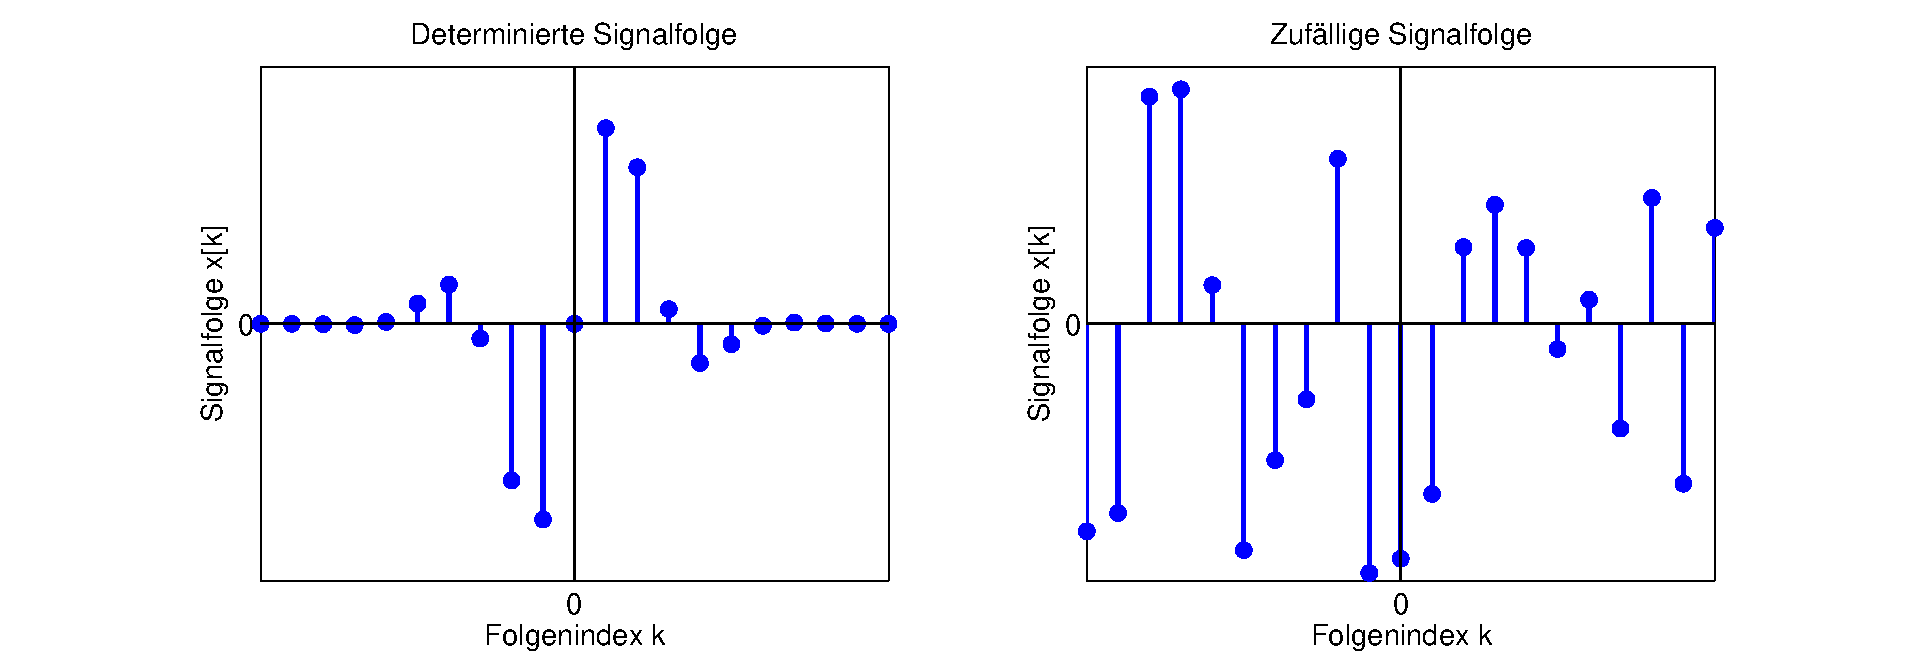
\includegraphics[width=1\textwidth]{Kapitel3/Bilder/image3.eps}}
  \caption{Beispiele für determinierte und zufällige Signalfolgen}
  \label{fig:DeterminierteZufaelligeFolgen}
\end{figure}

\subsubsection{Zeitlich begrenzte und kausale Signalfolgen}

\noindent Auch bei Signalfolgen wird oft mit einer zeitlichen Begrenzung gearbeitet, weil eine Signalfolge nur einen begrenzten Zeitraum lang beobachtet werden kann und weil zum Beispiel Impulsfolgen für die Charakterisierung von Systemen verwendet werden. Bild \ref{fig:BegrenzteKausaleFolgen} zeigt zeitlich begrenzte Signalfolgen.
\clearpage
\begin{figure}[H]
  \centerline{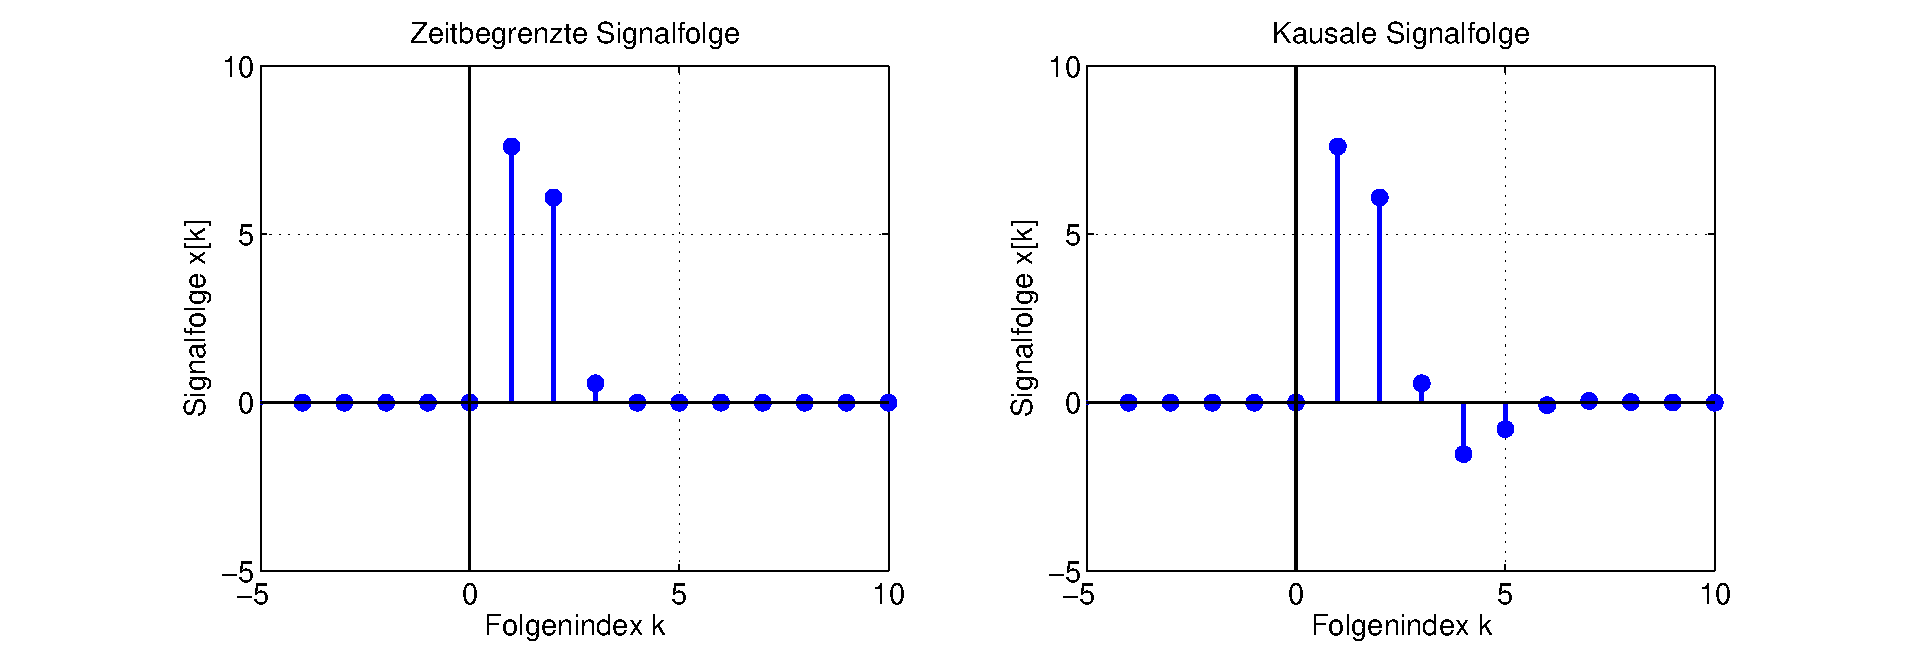
\includegraphics[width=1\textwidth]{Kapitel3/Bilder/image4.eps}}
  \caption{Darstellung einer beidseitig zeitbegrenzten und einer kausalen Signalfolge}
  \label{fig:BegrenzteKausaleFolgen}
\end{figure}

\noindent Beidseitig zeitbegrenzte Signalfolgen sind Signale, die nur f\"{u}r einen Bereich k$_{1}\mathrm{\le}$ k $\mathrm{<}$ k$_{2}$ von null verschieden sind. Einige Signale sind nur einseitig begrenzt, zum Beispiel ist ein f\"{u}r k = k$_{1}$ stattfindender Sprung nur einseitig zeitbegrenzt. Da diese Signalfolgen rechts auf dem Zeitstrahl von null verschieden sind, werden sie als rechtsseitige Signalfolgen bezeichnet. Eine spezielle rechtsseitige Signalfolge ist die kausale Signalfolge, f\"{u}r die gilt:

\begin{equation}\label{eq:threefour}
x\left[k\right]= 0\rm \; \; \; \text{für}\; k\; <{\rm \; 0}
\end{equation}

\noindent Damit gelten die Definitionen zeitkontinuierlicher Signale sinngem\"{a}{\ss} auch f\"{u}r Signalfolgen.

\subsubsection{Quadratisch summierbare Signalfolgen}

\noindent Für die Existenz von unendlichen Reihen zum Beispiel bei der Fourier-Transformation von Folgen oder der sogenannten z-Transformation ist der Begriff der Leistungs- und Energiesignalfolge wesentlich. Wie bei zeitkontinuierlichen Signalen wird von der Vorstellung ausgegangen, dass die an einem Widerstand umgesetzte Leistung proportional zum Quadrat der anliegenden Spannung u(t) beziehungsweise proportional zum Quadrat des durchfließenden Stromes i(t) ist.

\begin{equation}\label{eq:threefive}
p_{el} \left(t\right)=\frac{u^{2} \left(t\right)}{R} =i^{2} \left(t\right)\cdot R
\end{equation}

\noindent F\"{u}r zeitkontinuierliche Signale wird damit die Energie eines Signals berechnet zu

\begin{equation}\label{eq:threesix}
E=\int\limits _{-\infty }^{\infty }p_{el} \left(t\right){\rm \; }dt =\int\limits  _{-\infty }^{\infty }\frac{u^{2} \left(t\right)}{R} {\rm \; }dt =\int\limits  _{-\infty }^{\infty }i^{2} \left(t\right)\cdot R{\rm \; }dt 
\end{equation}

\noindent und vereinfachend zu der normierten Beschreibung 

\begin{equation}\label{eq:threeseven}
E=\int\limits _{-\infty }^{\infty }\left|x\left(t\right)\right|^{2} {\rm \; }dt 
\end{equation}

\noindent \"{u}bergegangen. Da f\"{u}r zeitdiskrete Signalfolgen keine Integration durchgef\"{u}hrt werden kann, wird f\"{u}r Signalfolgen die Summe

\begin{equation}\label{eq:threeeight}
E=\sum _{k=-\infty }^{\infty }\left|x\left[k\right]\right|^{2} 
\end{equation}

\noindent als Energie definiert. Mit dieser Definition k\"{o}nnen Signalfolgen wie zeitkontinuierliche Signale in Energiesignalfolgen und Leistungssignalfolgen eingestuft werden:\bigskip

{\fontfamily{phv}\selectfont
\noindent\textbf{Energiesignalfolgen}} \smallskip

\noindent Energiesignalfolgen haben eine von Null verschiedene und endliche Gesamtenergie in dem Intervall von - $\infty$ $\mathrm{<}$ k $\mathrm{<}$ $\infty$. Die mathematische Bedingung f\"{u}r Energiesignalfolgen lautet:

\begin{equation}\label{eq:threenine}
0<\sum _{k=-\infty }^{\infty }\left|x\left[k\right]\right|^{2}  <\infty 
\end{equation}

\noindent Diese Bedingung ist f\"{u}r jede zeitbegrenzte und amplitudenbegrenzte Folge erf\"{u}llt. Folgen, die gleichzeitig zeit- und amplitudenbegrenzt sind, sind damit immer Energiesignalfolgen. \bigskip

{\fontfamily{phv}\selectfont
\noindent\textbf{Leistungssignalfolgen}} \smallskip

\noindent Leistungssignalfolgen haben dagegen eine von Null verschiedene und endliche mittlere Leistung. Mathematisch ergibt sich folgende Definition f\"{u}r Leistungssignalfolgen:

\begin{equation}\label{eq:threeten}
0\le {\mathop{\lim }\limits_{K\to \infty }} \frac{1}{K} \cdot \sum _{k=-K}^{K}\left|x\left[k\right]\right|^{2}  <\infty 
\end{equation}

\noindent F\"{u}r Signalfolgen mit einer begrenzten Amplitude bedeutet das, dass sie nicht zeitbegrenzt sein m\"{u}ssen. Ihre Energie ist zwar unendlich, ihre Energie im Intervall von - K bis K ist aber begrenzt. 

\noindent Signalfolgen, die weder Energie- noch Leistungssignalfolgen sind, spielen in der Systemtheorie praktisch keine Rolle, da technische Vorg\"{a}nge grunds\"{a}tzlich mit endlichen Gr\"{o}{\ss}en verbunden sind.

\subsubsection{Symmetrieeigenschaften von Signalfolgen}

\noindent Die Bestimmung von Signaleigenschaften und Transformationen von Signalfolgen kann wie bei zeitkontinuierlichen Signalen durch Ausnutzen von Symmetrien vereinfacht werden. Deshalb werden Symmetrieeigenschaften diskutiert, mit denen Signalfolgen in gerade und ungerade Signalfolgen eingeteilt werden k\"{o}nnen. Gerade Signalfolgen sind f\"{u}r alle k symmetrisch zur Achse k = 0, also zur Ordinatenachse. F\"{u}r eine gerade Signalfolge gilt deshalb die Bedingung:

\begin{equation}\label{eq:threeeleven}
x\left[k\right]=x\left[-k\right]
\end{equation}

\noindent Eine kosinusf\"{o}rmige Signalfolge mit einem Nullphasenwinkel $\varphi$ = 0 ist ein Beispiel f\"{u}r eine gerade Signalfolge, denn es gilt:

\begin{equation}\label{eq:threetwelve}
x\left[k\right]=\cos \left(\frac{2\cdot \pi }{T_{0} } \cdot T_{A} \cdot k\right)=\cos \left(-\frac{2\cdot \pi }{T_{0} } \cdot T_{A} \cdot k\right)=x\left[-k\right]
\end{equation}

\noindent Ungerade Signalfolgen sind f\"{u}r alle k punktsymmetrisch zu dem Koordinatenursprung (0{\textbar}0). Dies kann mathematisch ausgedr\"{u}ckt werden als

\begin{equation}\label{eq:threethirteen}
x\left[k\right]=-x\left[-k\right]
\end{equation}

\clearpage

\noindent Eine sinusf\"{o}rmige Signalfolge ist ein Beispiel f\"{u}r eine ungerade Signalfolge, denn es gilt:

\begin{equation}\label{eq:threefourteen}
x\left[k\right]=\sin \left(\frac{2\cdot \pi }{T_{0} } \cdot T_{A} \cdot k\right)=-\sin \left(-\frac{2\cdot \pi }{T_{0} } \cdot T_{A} \cdot k\right)=-x\left[-k\right]
\end{equation}

\noindent Bild \ref{fig:GeardeUngeradeFolgen}  zeigt Kosinus- und Sinusfolgen als Beispiele f\"{u}r gerade und ungerade Signalfolgen. 

\begin{figure}[H]
  \centerline{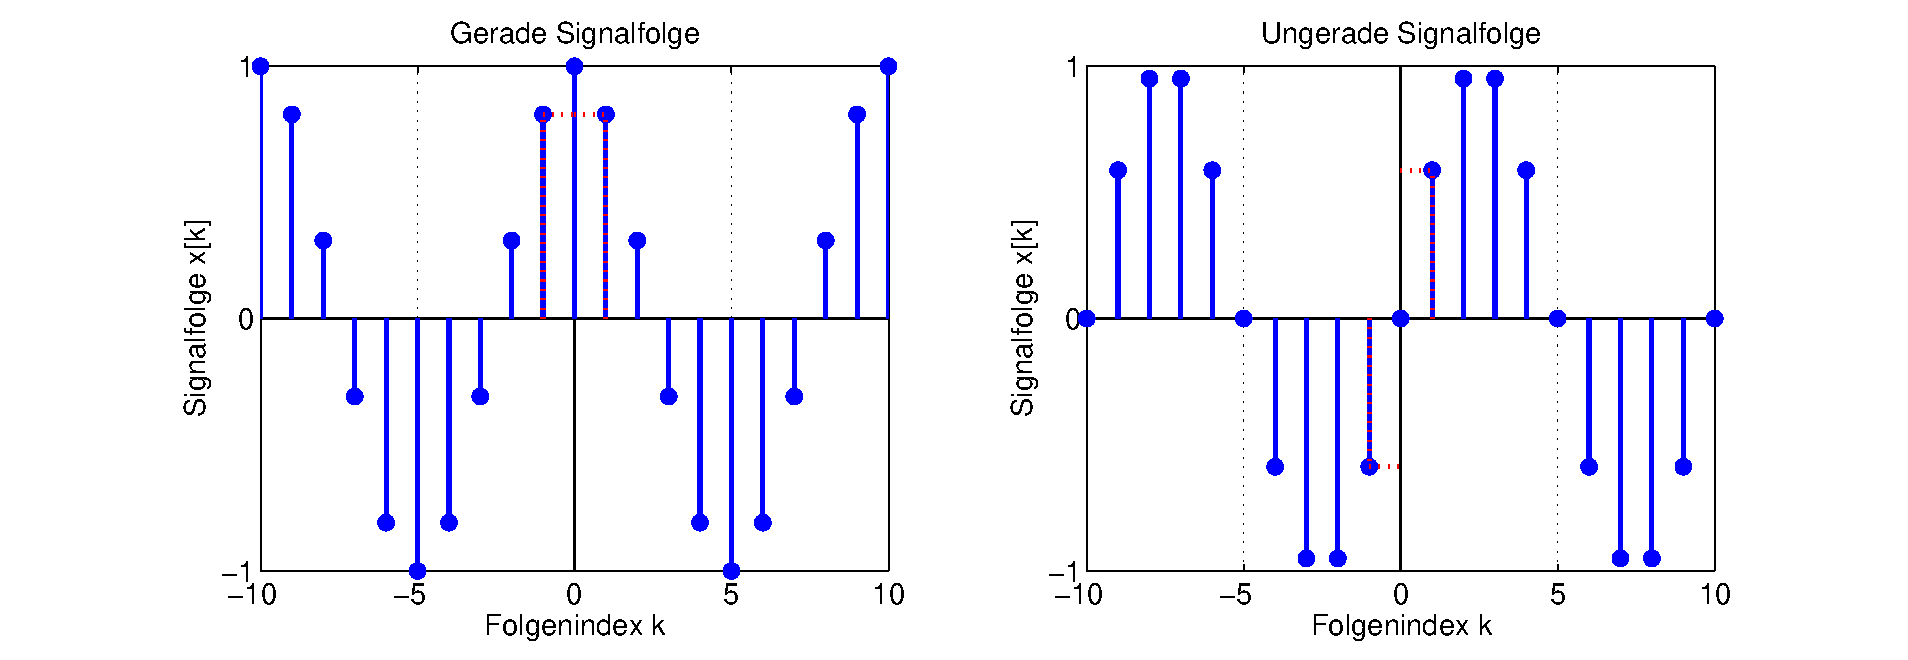
\includegraphics[width=1\textwidth]{Kapitel3/Bilder/image5.eps}}
  \caption{Kosinus- und Sinusfolgen als Beispiele für gerade und ungerade Signalfolgen}
  \label{fig:GeardeUngeradeFolgen}
\end{figure}

\noindent Es existieren Signalfolgen, die weder gerade, noch ungerade sind, sie weisen keine Symmetrie auf. Jede beliebige Signalfolge l\"{a}sst sich aber in einen geraden und einen ungeraden Anteil aufspalten. 

\begin{equation}\label{eq:threefivteen}
x\left[k\right]=x_{g} \left[k\right]+x_{u} \left[k\right]
\end{equation}

\noindent wobei sich die beiden Anteile ergeben aus

\begin{equation}\label{eq:threesixteen}
x_{g} \left[k\right]=\frac{1}{2} \cdot \left(x\left[k\right]+x\left[-k\right]\right)
\end{equation}

\noindent und

\begin{equation}\label{eq:threeseventeen}
x_{u} \left[k\right]=\frac{1}{2} \cdot \left(x\left[k\right]-x\left[-k\right]\right)
\end{equation}

\noindent Bild \ref{fig:GeraderUngeraderAnteil} verdeutlicht die Zerlegung eines Signals in einen geraden und einen ungeraden Anteil an einem Beispiel.

\begin{figure}[H]
  \centerline{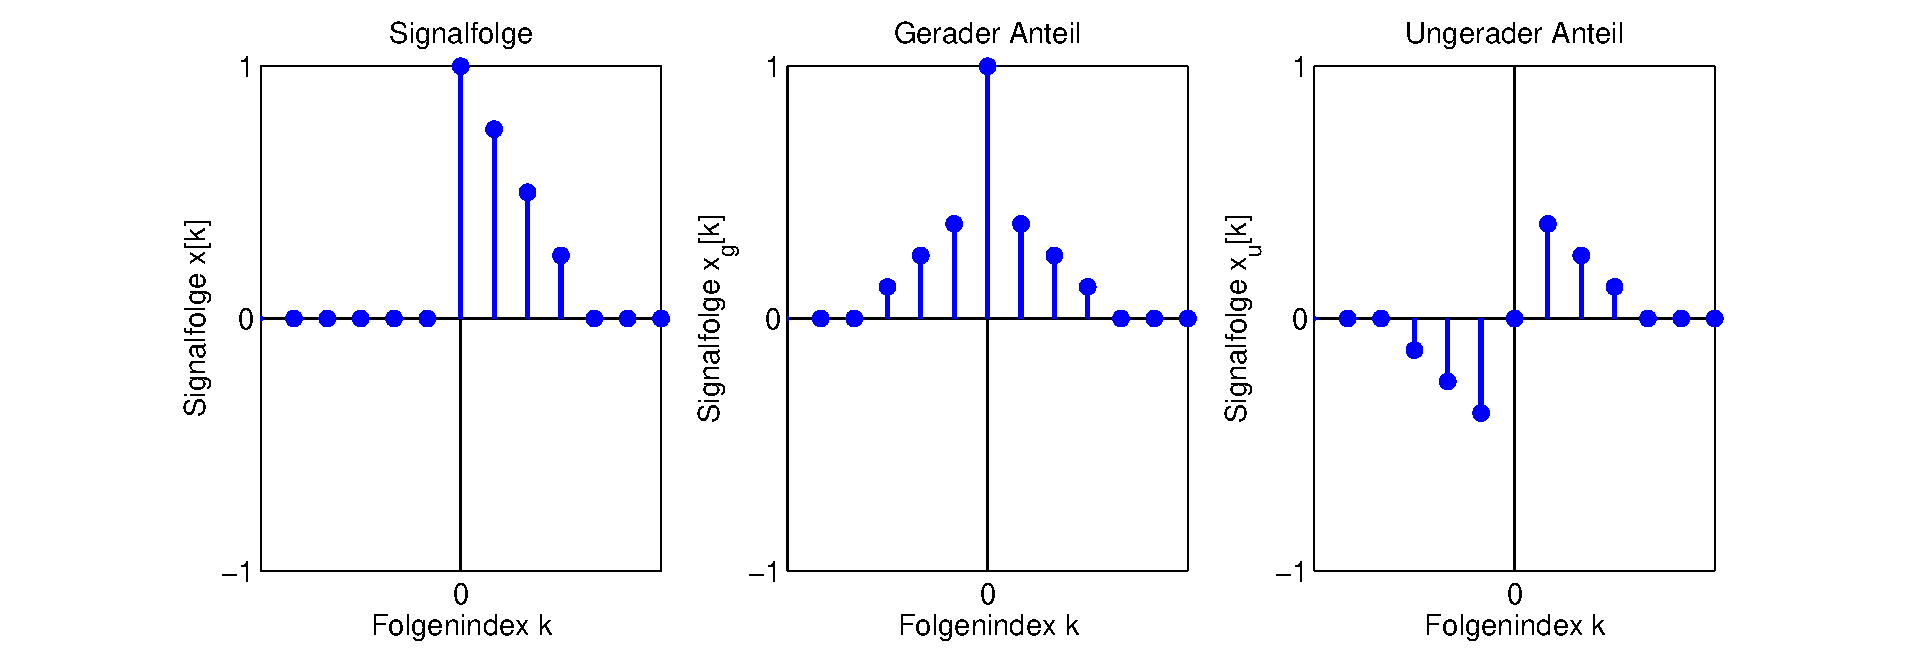
\includegraphics[width=1\textwidth]{Kapitel3/Bilder/image6.eps}}
  \caption{Zerlegung einer Signalfolge in geraden und ungeraden Anteil}
  \label{fig:GeraderUngeraderAnteil}
\end{figure}

\clearpage

\subsubsection{Zusammenfassung Eigenschaften von Signalfolgen}

\noindent Zur besseren Übersicht sind in Tabelle \ref{tab:threeone} die diskutierten Eigenschaften für Signalfolgen darge-stellt. 

\begin{table}[H]
\setlength{\arrayrulewidth}{.1em}
\caption{Tabellarische Übersicht über Signaleigenschaften für Signalfolgen}
\setlength{\fboxsep}{0pt}%
\colorbox{lightgray}{%
\arrayrulecolor{white}%
\begin{tabular}{| l | l |}
\hline
\parbox[c][0.28in][c]{3in}{\smallskip\centering\textbf{\fontfamily{phv}\selectfont{Signaleigenschaft}}} & 
\parbox[c][0.28in][c]{3in}{\smallskip\centering\textbf{\fontfamily{phv}\selectfont{Mathematische Beschreibung}}}\\ \hline
\parbox[c][1in][c]{3in}{\centering{\fontfamily{phv}\selectfont{Explizit definierte Signalfolge}}}
& \parbox[c][1in][c]{3in}{\centering{\fontfamily{phv}\selectfont{Folgenwert kann direkt abgelesen werden, \\
zum Beispiel\\
$x\left[k\right]=10\cdot r^{k} \cdot \sin \left(\Omega _{0} \cdot k\right)$
}}}\\ \hline 

\parbox[c][1in][c]{3in}{\centering{\fontfamily{phv}\selectfont{Implizit definierte Signalfolge}}} 
& \parbox[c][1in][c]{3in}{\centering{\fontfamily{phv}\selectfont{Folgenwert muss berechnet werden,\\
zum Beispiel\\
$x\left[k-1\right]+3\cdot x\left[k-2\right]=5\cdot x\left[k\right]$\\
mit Anfangsbedingung x[0] = x${}_{0}$
}}}\\ \hline


\parbox[c][0.64in][c]{3in}{\centering{\fontfamily{phv}\selectfont{Begrenzte Signalfolge}}} & 
\parbox[c][0.64in][c]{3in}{\centering{\fontfamily{phv}\selectfont{$x\left[k\right]=0 \; \;\; \; \text{für} \; \; k<k_{1} \; \; \text{und/oder} \; \; k>k_{2} $}}}\\ \hline

\parbox[c][0.64in][c]{3in}{\centering{\fontfamily{phv}\selectfont{Kausale Signalfolge}}} & 
\parbox[c][0.64in][c]{3in}{\centering{\fontfamily{phv}\selectfont{\fontfamily{phv}\selectfont{$x\left[k\right]=0\; \;\; \; \text{für}\; \; k<0$}}}}\\ \hline

\parbox[c][0.8in][c]{3in}{\centering{\fontfamily{phv}\selectfont{Energiesignalfolge}}} & 
\parbox[c][0.8in][c]{3in}{\centering{$0<\sum _{k=-\infty }^{\infty }\left|x\left[k\right]\right|^{2}  <\infty $}}\\ \hline

\parbox[c][0.64in][c]{3in}{\centering{\fontfamily{phv}\selectfont{Leistungssignalfolge}}} 
& \parbox[c][0.64in][c]{3in}{\centering{$0\le {\mathop{\lim }\limits_{K\to \infty }} \frac{1}{K} \cdot \sum _{k=-K}^{K}\left|x\left[k\right]\right|^{2}  <\infty $}}\\ \hline

\parbox[c][0.64in][c]{3in}{\centering{\fontfamily{phv}\selectfont{Gerade Signalfolge}}} & \parbox[c][0.64in][c]{3in}{\centering{$x\left[k\right]=x\left[-k\right]$}}\\ \hline

\parbox[c][0.64in][c]{3in}{\centering{\fontfamily{phv}\selectfont{Ungerade Signalfolge}}} & 
\parbox[c][0.64in][c]{3in}{\centering{$x\left[k\right]=-x\left[-k\right]$}}\\ \hline

\parbox[c][0.64in][c]{3in}{\centering{\fontfamily{phv}\selectfont{Gerader Anteil}}} & \parbox[c][0.64in][c]{3in}{\centering{$x_{g} \left[k\right]=\frac{1}{2} \cdot \left(x\left[k\right]+x\left[-k\right]\right)$}}\\ \hline

\parbox[c][0.64in][c]{3in}{\centering{\fontfamily{phv}\selectfont{Ungerader Anteil}}} & \parbox[c][0.64in][c]{3in}{\centering{$x_{u} \left[k\right]=\frac{1}{2} \cdot \left(x\left[k\right]-x\left[-k\right]\right)$}}\\ \hline

\end{tabular}%
}
\label{tab:threeone}
\end{table}

\clearpage

\subsection{Sprung- und Impulsfolgen}

\noindent Auch bei der Beschreibung und Interpretation von zeitdiskreten Systemen werden Impuls- und Sprungantworten verwendet. Deshalb werden in diesem Abschnitt Sprung- und Impulsfolgen vorgestellt, weitere Signalfolgen daraus abgeleitet und das Rechnen mit Impulsfolgen vertieft.

\subsubsection{Impulsfolge}

\noindent Die Impulsfolge ist im Gegensatz zur Impulsfunktion nicht als Grenzwert definiert, sondern durch die Bedingung

\begin{equation}\label{eq:threeeighteen}
\delta \left[k\right]=\left\{\begin{array}{l} {
1\quad \text{ für } \; k\; =\; 0} \\ 
{0\quad \text{ für ganzzahlige }\; \; k\; \ne \rm \; 0} \end{array}\right.
\end{equation}

\noindent Im Vergleich zur Impulsfunktion ist die Impulsfolge nicht unendlich hoch, sondern hat eine Höhe, die beim kontinuierlichen System dem Gewicht der Impulsfunktion entspricht. Diese Defini-tion erleichtert das Rechnen mit der Impulsfolge im Vergleich zur Impulsfunktion. Bild \ref{fig:ImpulsFunktion} stellt die Impulsfolge grafisch dar.

\begin{figure}[H]
  \centerline{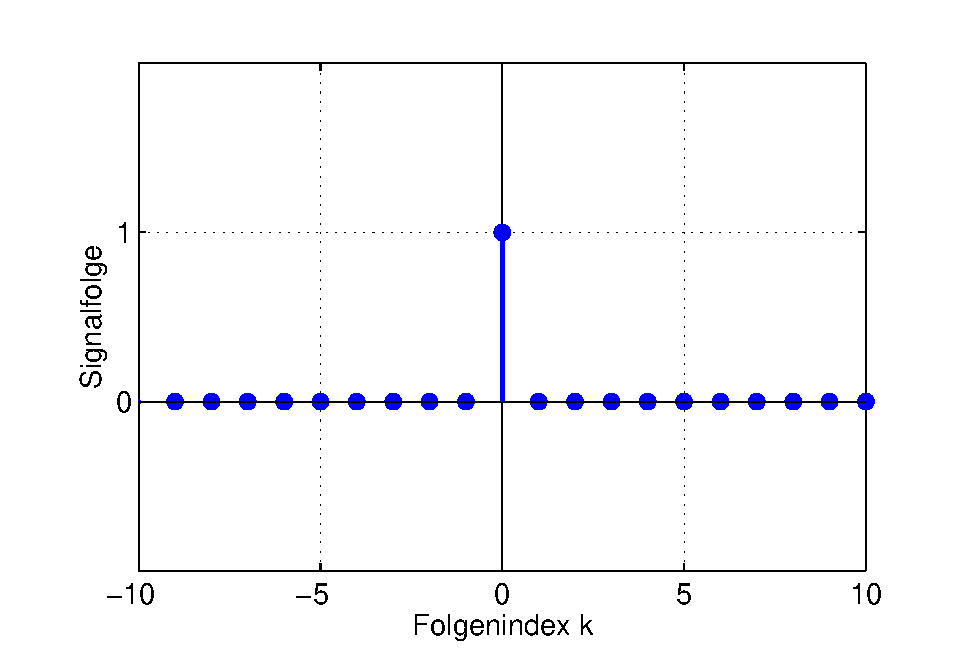
\includegraphics[width=0.5\textwidth]{Kapitel3/Bilder/image7.eps}}
  \caption{Darstellung der Impulsfolge $\delta$[k]}
  \label{fig:ImpulsFunktion}
\end{figure}

\noindent Die Impulsfolge wird f\"{u}r die Charakterisierung von Systemen verwendet. Die Impulsfolge ist sowohl zeitlich, als auch von der Amplitude begrenzt. Sie ist eine Energiesignalfolge. Da die Impulsfolge f\"{u}r k $\mathrm{<}$ 0 null ist, ist sie eine kausale Folge. Da praktisch alle Werte der Impulsfolge null sind bis auf den Wert, an dem das Argument der Impulsfolge zu null wird, ergibt sich die Summe \"{u}ber die Impulsfolge zu

\begin{equation}\label{eq:threenineteen}
\sum _{k=-\infty }^{\infty }\delta \left[k\right] =1
\end{equation}

\noindent Mit der Impulsfolge werden zwei wichtige Methoden realisiert, die f\"{u}r die Darstellung abgetasteter Signale notwendig sind. 

\clearpage


{\fontfamily{phv}\selectfont
\noindent\textbf{Ausblendeigenschaft der Impulsfolge}} \smallskip

\noindent Mit Hilfe der Impulsfolge können einzelne Werte einer Folge x[k] selektiert werden. 

\begin{equation}\label{eq:threetwenty}
\sum _{k=-\infty }^{\infty }x\left[k\right]\cdot \delta \left[k-k_{0} \right] =x\left[k_{0} \right]
\end{equation}

\noindent Diese Bedingung ergibt sich daraus, dass die Impulsfolge f\"{u}r alle Werte von k zu null wird, au{\ss}er f\"{u}r den Wert $k = k{}_{0}$. F\"{u}r $k = k{}_{0}$ nimmt die Impulsfolge den Wert 1 an, die Folge x[k] hat f\"{u}r $k = k{}_{0}$ den Wert $x[k{}_{0}]$. \bigskip

{\fontfamily{phv}\selectfont
\noindent\textbf{Periodische Impulsfolge}} \smallskip

\noindent Insbesondere bei der Darstellung periodischer Signale wird die periodische Impulsfolge einge-setzt. 

\begin{equation}\label{eq:threetwentyone}
x\left[k\right]=\sum _{n=-\infty }^{\infty }\delta \left[k-n\cdot K_{0} \right]
\end{equation}

\noindent Jede Impulsfolge ist an allen Stellen null, bis auf die Stelle k = n$\cdot$K${}_{0}$. Durch die Summe entsteht eine in K periodische Impulsfolge, die in Bild \ref{fig:ImpulsfolgePeriodisch} dargestellt ist. Sie wird auch als Impulskamm bezeichnet.

\begin{figure}[H]
  \centerline{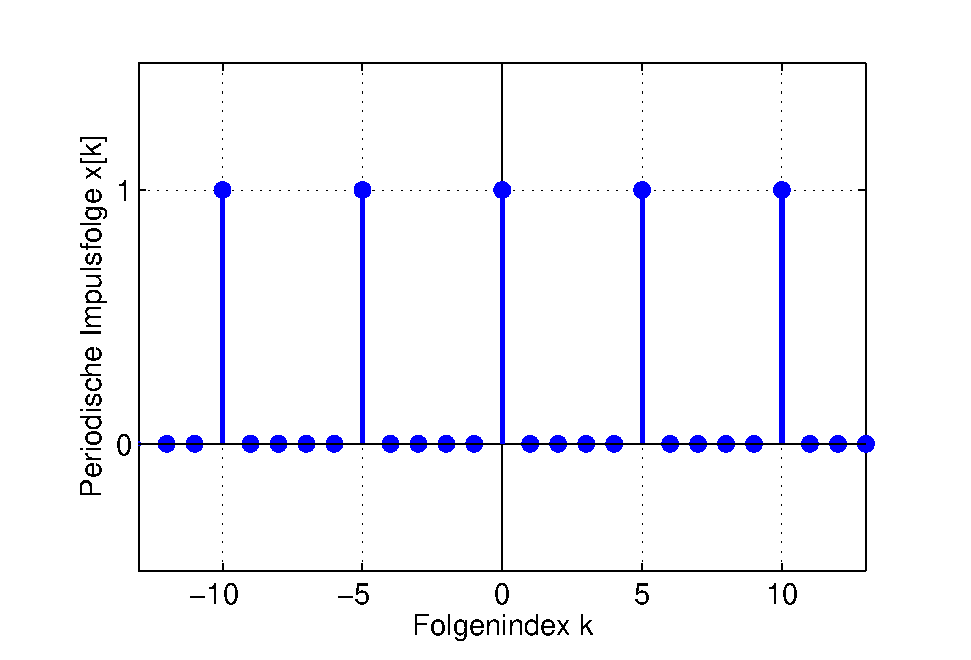
\includegraphics[width=0.5\textwidth]{Kapitel3/Bilder/image8.eps}}
  \caption{Darstellung der in K${}_{0}$ = 5 periodischen Impulsfolge}
  \label{fig:ImpulsfolgePeriodisch}
\end{figure}

\subsubsection{Sprungfolge}

\noindent Die Sprungfolge $\sigmaup$[k] ist identisch zur Sprungfunktion im zeitkontinuierlichen Bereich definiert als 

\begin{equation}\label{eq:threetwentytwo}
\sigma \left[k\right]=\left\{\begin{array}{l} {0\quad \text{für}\rm \;\; k<0} \\ {1\quad \text{für} \rm \;\; k\ge 0} \end{array}\right.
\end{equation}

\noindent Wie im zeitkontinuierlichen Bereich ist die Sprungfolge eine wichtige Testfolge. Bild \ref{fig:Sprungfolge} stellt die Sprungfolge dar.

\clearpage

\begin{figure}[H]
  \centerline{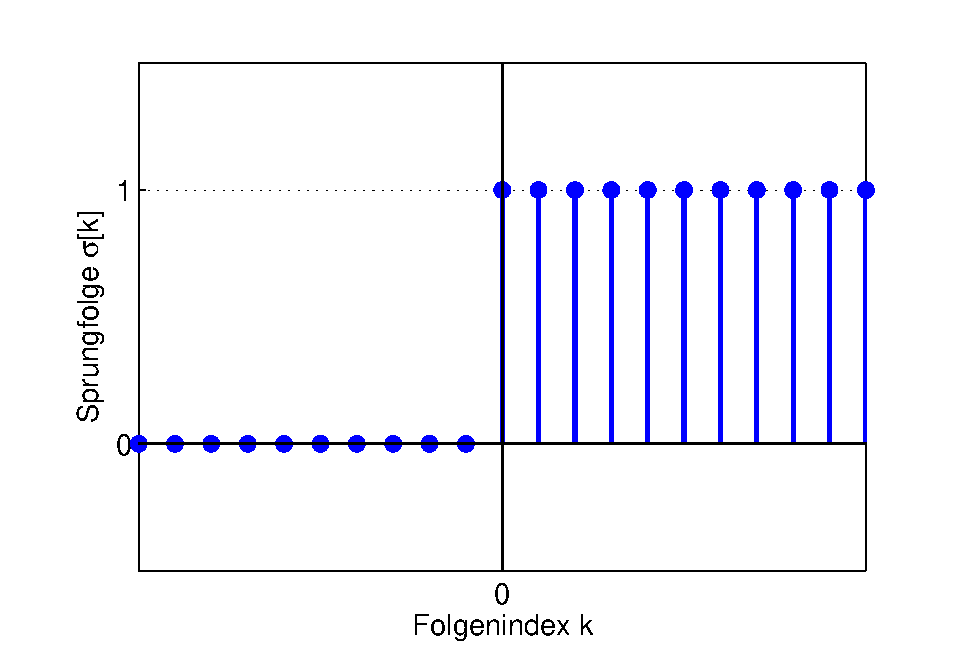
\includegraphics[width=0.5\textwidth]{Kapitel3/Bilder/image9.eps}}
  \caption{Darstellung der diskreten Sprungfolge $\sigma$[k]}
  \label{fig:Sprungfolge}
\end{figure}

\noindent Die Sprungfolge wird zum Beispiel daf\"{u}r verwendet, ideale Einschaltvorg\"{a}nge zu beschreiben. Die Sprungfolge ist zeitlich nicht begrenzt und ist damit keine Energiesignalfolge. Wegen ihrer begrenzten Amplitude ist die Bedingung f\"{u}r eine Leistungssignalfolge erf\"{u}llt. Da die Sprungfolge f\"{u}r k $\mathrm{<}$ 0 null ist, ist sie eine kausale Folge.

\noindent Sprung- und Impulsfolge k\"{o}nnen in Abh\"{a}ngigkeit voneinander dargestellt werden. So kann die Sprungfolge als Summe einzelner verschobener Impulse dargestellt werden.

\begin{equation}\label{eq:threetwentythree}
\sigma \left[k\right]=\sum _{\kappa =0}^{\infty }\delta \left[k-\kappa \right]
\end{equation}

\noindent Andererseits ist die Impulsfolge die Differenz zweier Sprungfolgen, die um einen Index $k{}_{0} = 1$ gegeneinander verschoben sind.

\begin{equation}\label{eq:threetwentyfour}
\delta \left[k\right]=\sigma \left[k\right]-\sigma \left[k-1\right]
\end{equation}

\noindent Aus dem Vergleich mit der Abh\"{a}ngigkeit der zeitkontinuierlichen Sprung- und Impulsfunktion ergibt sich ein weiterer interessanter Aspekt: Die Sprungfunktion kann als Integral der Impulsfunktion dargestellt werden. Im zeitdiskreten Bereich wird das Integral durch die Summe ersetzt.

\begin{equation}\label{eq:threetwentyfive}
\sigma \left[k\right]=\sum _{\kappa =-\infty }^{k}\delta \left[\kappa \right]
\end{equation}

\noindent In zeitkontinuierlichen Bereich ist die Impulsfunktion die Ableitung der Sprungfunktion. Im zeitdiskreten Bereich wird die Ableitung durch den Differenzenquotienten ersetzt, sodass gilt:

\begin{equation}\label{eq:threetwentysix}
\delta \left[k\right]=\frac{\sigma \left[k\right]-\sigma \left[k-1\right]}{k-(k-1)} =\sigma \left[k\right]-\sigma \left[k-1\right]
\end{equation}

\noindent Im zeitdiskreten Bereich gehen also das Integral in eine Summe und die Ableitung in einen Differenzenquotienten \"{u}ber.

\clearpage

\subsubsection{Integral abgetasteter Signale}

\noindent Ideal abgetastete Signale können als Summe gewichteter Impulse dargestellt werden. 

\begin{equation}\label{eq:threetwentyseven}
x_{A} \left(t\right)=\sum _{k=-\infty }^{\infty }x\left(k\cdot T_{A} \right)\cdot \delta \left(t-k\cdot T_{A} \right) =\sum _{k=-\infty }^{\infty }x\left[k\right]\cdot \delta \left(t-k\cdot T_{A} \right) 
\end{equation}

\noindent Insbesondere bei der Berechnung des Spektrums abgetasteter Signale werden Integrale berechnet, in denen ideal abgetasteten Signale vorkommen. Als Vorbereitung dazu wird das Integral abgetasteter Signale berechnet. 

\begin{equation}\label{eq:threetwentyeight}
\int\limits _{\tau =-\infty }^{t}x_{A} \left(\tau \right)\, \, d\tau  =\int\limits _{\tau =-\infty }^{t}\sum _{\kappa =-\infty }^{\infty }x\left[\kappa \right]\cdot \delta \left(\tau -\kappa \cdot T_{A} \right) \, \, d\tau  =\sum _{\kappa =-\infty }^{\infty }x\left[\kappa \right]\cdot \int\limits _{\tau =-\infty }^{t}\delta \left(\tau -\kappa \cdot T_{A} \right)\, \, d\tau 
\end{equation}

\noindent Um von dem zeitkontinuierlichen Integralausdruck zu einer Summe zu kommen, wird die Zeitvariable normiert.

\begin{equation}\label{eq:threetwentynine}
\tau =T_{A} \cdot \eta 
\end{equation}

\noindent Aus der Substitutionsregel folgt 

\begin{equation}\label{eq:threethirty}
d\tau =T_{A} \cdot d\eta 
\end{equation}

\noindent F\"{u}r die Zeitpunkte t = k$\cdot$T${}_{A}$ ergibt sich 

\begin{equation}\label{eq:threethirtyone}
\sum _{\kappa =-\infty }^{\infty }x\left[\kappa \right]\int\limits _{\eta =-\infty }^{k}\delta \left(\eta -\kappa \right)\cdot T_{A} \, \, d\eta   =\sum _{\kappa =-\infty }^{\infty }x\left[\kappa \right]\cdot T_{A} \cdot \int\limits _{\eta =-\infty }^{k}\delta \left(\eta -\kappa \right)\, \, d\kappa  
\end{equation}

\noindent Das Integral bewirkt, dass nur Werte aufsummiert werden, die kleiner oder gleich k sind. Damit kann der Ausdruck umgeformt werden zu

\begin{equation}\label{eq:threethirtytwo}
\sum _{\kappa =-\infty }^{\infty }x\left[\kappa \right]\cdot T_{A} \cdot \int _{\eta =-\infty }^{k}\delta \left(\eta -\kappa \right)\, \, d\kappa   =T_{A} \cdot \sum _{\kappa =-\infty }^{k}x\left[\kappa \right]\cdot \delta \left[k-\kappa \right]
\end{equation}

\noindent Der Vergleich zeigt, dass bei der Berechnung von Integralen ideal abgetasteter Signale neben der Summe der Abtastwerte die Abtastzeit ber\"{u}cksichtigt werden muss. 

\noindent Tabelle \ref{tab:twothree} vergleicht die Definition und die Eigenschaften der Impulsfolge und der Impulsfunktion tabellarisch miteinander.

\clearpage

\begin{table}[H]
\setlength{\arrayrulewidth}{.1em}
\caption{Tabellarische Zusammenfassung der wesentlichen Eigenschaften der Impulsfunktion}
\setlength{\fboxsep}{0pt}%
\colorbox{lightgray}{%
\arrayrulecolor{white}%
\begin{tabular}{| wc{5.6cm} | wc{5.5cm} | wc{5.5cm} |}
\hline\xrowht{15pt}
{\fontfamily{phv}\selectfont
\textbf{Eigenschaft}} & 
{\fontfamily{phv}\selectfont
\textbf{Zeitkontinuierlicher Bereich}} &
{\fontfamily{phv}\selectfont
\textbf{Zeitdiskreter  Bereich}}\\ \hline \xrowht{40pt}

\fontfamily{phv}\selectfont{Definition des Impulses} &
$\delta (t)={\mathop{\lim }\limits_{\varepsilon \to 0}} {\rm \; }\frac{1}{\varepsilon } \cdot \left(\sigma \left(t+\frac{\varepsilon }{2} \right)-\sigma \left(t-\frac{\varepsilon }{2} \right)\right)$ & $\delta \left[k\right]=\left\{\begin{array}{l} {1 \quad  \text{für} \; k\; =\; 0} \\ {0\quad \text{für} k \ne {\rm \; 0}} \end{array}\right. $ \\ \hline \xrowht{40pt}

\fontfamily{phv}\selectfont{Integration} &
$\int\limits_{-\infty }^{\infty }\delta \left(\tau \right){\rm \; }d\tau  =1$ & $\sum _{k=-\infty }^{\infty }\delta \left[k\right] =1$  \\ \hline\xrowht{40pt}

\fontfamily{phv}\selectfont{Ausblendeigenschaft}  &
$\int\limits _{-\infty }^{\infty }x\left(t\right)\cdot \delta \left(t-t_{0} \right){\rm \; }dt =x\left(t_{0} \right)$ & 
$\sum _{k=-\infty }^{\infty }x\left[k\right]\cdot \delta \left[k-k_{0} \right] =x\left[k_{0} \right]$ \\ \hline\xrowht{40pt}

\fontfamily{phv}\selectfont{Impuls als Ableitung des Sprungs} & 
$\delta \left(t\right)=\frac{d\sigma }{dt} $ & 
$\delta \left[k\right]=\sigma \left[k\right]-\sigma \left[k-1\right]$ \\ \hline \xrowht{40pt}

\fontfamily{phv}\selectfont{Sprung als Integral des Impulses} & 
$\sigma \left(t\right)=\int\limits _{-\infty }^{t}\delta \left(\tau \right){\rm \; }d\tau  $ & 
$\sigma \left[k\right]=\sum _{\kappa =-\infty }^{k}\delta \left[\kappa \right] $ \\ \hline \xrowht{40pt}

\fontfamily{phv}\selectfont{Integral eines abgetasteten Signals}  & 
\multicolumn{2}{c|}{$\int\limits _{\tau =-\infty }^{t}x_{A} \left(\tau \right)\, \, d\tau  =T_{A} \cdot \sum _{\kappa =-\infty }^{k}x\left[\kappa \right]\cdot \delta \left[k-\kappa \right] $} \\ \hline 
\end{tabular}%
}
\label{tab:twothree}
\end{table}

\subsubsection{Rechteckfolge}

\noindent Die Rechteckfolge ist abschnittsweise definiert als 

\begin{equation}\label{eq:threethirtythree}
x\left[k\right]=\left\{\begin{array}{l} {0\quad \text{für} \quad \text{k}<-\, K} \\ {1\rm \quad \text{für} \quad -K\le \text{k}\rm \;<\rm \;K+1} \\ 
0\quad \text{für}\quad K+1 \rm \;\le \rm \;\text{k} \rm \; \end{array}\right.
\end{equation}

\noindent Die Rechteckfolge ist eine Folge mit endlicher Amplitude und endlicher Dauer. Die Bedingung f\"{u}r eine Energiesignalfolge ist deshalb erf\"{u}llt. Die Rechteckfolge nach Gleichung \eqref{eq:threethirtythree} ist keine kausale Folge, da sie f\"{u}r k $\mathrm{<}$ 0 nicht null ist. Durch eine Verschiebung um K nach rechts wird die Folge kausal. Beide Folgen sind in Bild \ref{fig:Rechteckfolgen} dargestellt.

\begin{figure}[H]
  \centerline{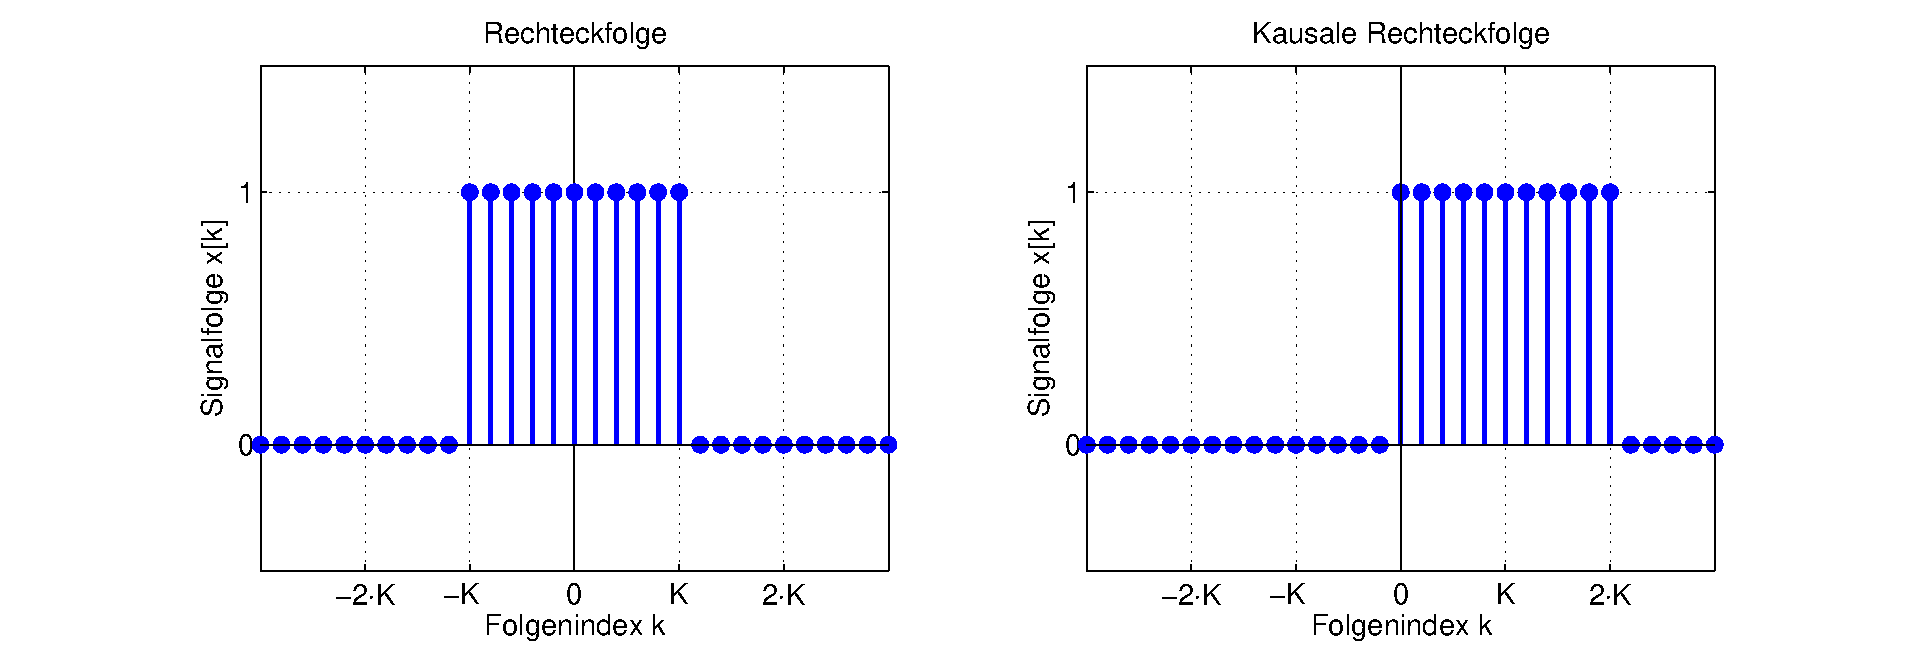
\includegraphics[width=1\textwidth]{Kapitel3/Bilder/image10.eps}}
  \caption{Rechteckfolge und verschobene Rechteckfolge}
  \label{fig:Rechteckfolgen}
\end{figure}

\clearpage

\noindent Die Rechteckfolge kann neben der abschnittsweisen Definition auch als Summe zweier Sprungfolgen dargestellt werden, die um - K beziehungsweise K + 1 verschoben sind.

\begin{equation}\label{eq:threethirtyfour}
x\left[k\right]=\sigma \left[k+K\right]-\sigma \left[k-\left(K+1\right)\right]=\sigma \left[k+K\right]-\sigma \left[k-K-1\right]
\end{equation}

\subsubsection{Signum-Folge}

\noindent Die Signum-Folge sgn[k] ist abschnittsweise definiert als

\begin{equation}\label{eq:threethirtyfive}
x\left[k\right]=sgn\left[k\right]=\left\{\begin{array}{l} {-{\rm 1}\quad \text{für k} <0} \\ 
{+1\quad \text{für k} \ge {\rm 0\; }} \end{array}\right.
\end{equation}

\noindent Auch die Signum-Folge kann mit Hilfe der Sprungfolge dargestellt werden.

\begin{equation}\label{eq:threethirtysix}
x\left[k\right]=sgn\left[k\right]=2\cdot \sigma \left[k\right]-1
\end{equation}

\noindent Bild \ref{fig:Rampenfolge} stellt die Signum-Folge grafisch dar. Sie dauert unendlich lange an und ist deshalb keine Energiesignalfolge. Wegen ihrer konstanten Amplitude ist die Bedingung f\"{u}r eine Leistungssignalfolge erf\"{u}llt. Die Signum-Folge ist nicht kausal und kann durch eine zeitliche Verschiebung auch nicht kausal werden.

\begin{figure}[H]
  \centerline{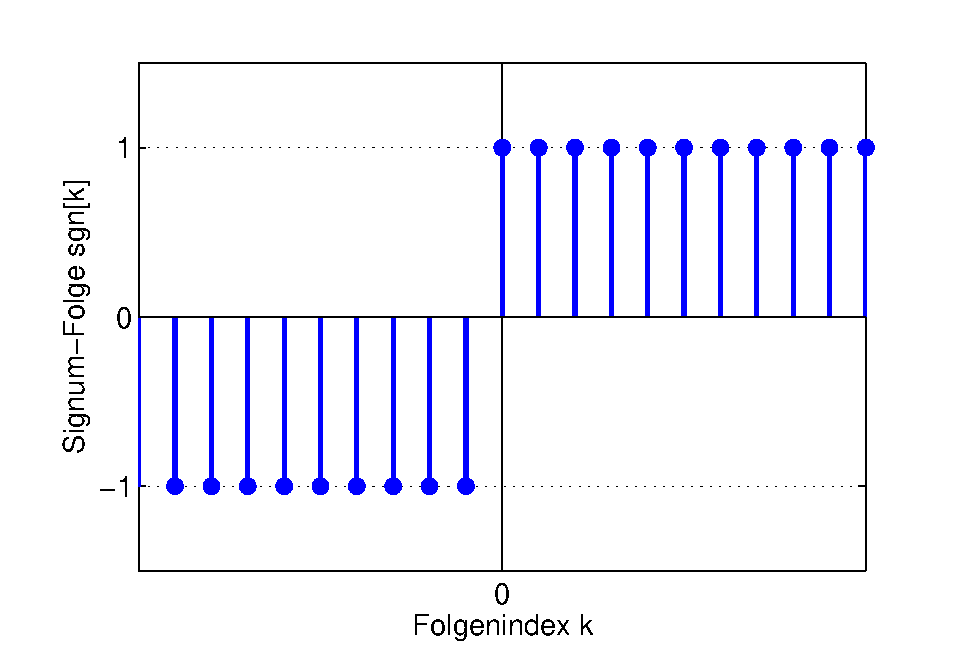
\includegraphics[width=0.5\textwidth]{Kapitel3/Bilder/image11.eps}}
  \caption{Signum-Folge sgn[k]}
  \label{fig:SignumFolge}
\end{figure}

\subsubsection{Rampenfolge}

\noindent Die Rampenfolge ist wie im zeitkontinuierlichen Bereich definiert als

\begin{equation}\label{eq:threethirtyseven}
x\left[k\right]=\left\{\begin{array}{l} {0\quad \text{für k} <0} \\ 
{\text{k}\quad \text{für k} \ge \rm \; 0} \end{array}\right. 
\end{equation}

\noindent Bild \ref{fig:Rampenfolge} stellt die Rampenfolge grafisch dar.

\begin{figure}[H]
  \centerline{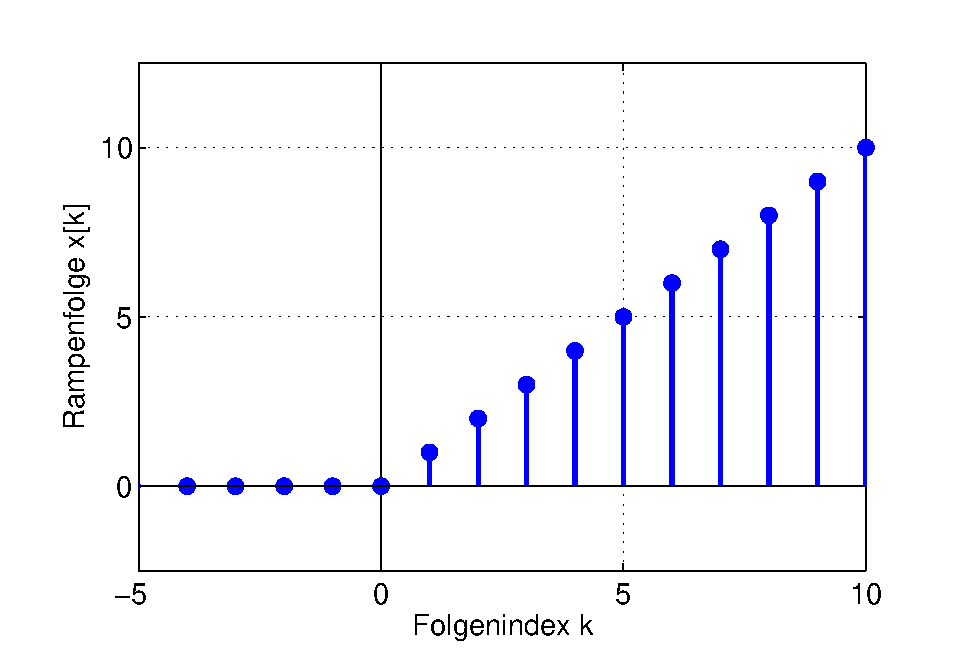
\includegraphics[width=0.5\textwidth]{Kapitel3/Bilder/image12.eps}}
  \caption{Rampenfolge}
  \label{fig:Rampenfolge}
\end{figure}

\noindent Die Rampenfolge kann als Summation \"{u}ber die Sprungfolge beschrieben werden. Dabei muss jedoch beachtet werden, dass die Rampenfolge an der Stelle k = 0 null ist. Deshalb muss die Rampenfolge dargestellt werden als 

\begin{equation}\label{eq:threethirtyeight}
x\left[k\right]=\sum _{\kappa =-\infty }^{k-1}\sigma \left[\kappa \right] =\sum _{\kappa =-\infty }^{k}\sigma \left[\kappa -1\right]
\end{equation}

\noindent Auswerten der Summengleichung führt zu der Darstellung

\begin{equation}\label{eq:threethirtynine}
x\left[k\right]=k\cdot \sigma \left[k\right]
\end{equation}

\noindent Die Rampenfolge hat weder eine begrenzte Amplitude, noch eine begrenzte Zeitdauer, sie ist weder Energie- noch Leistungssignalfolge. Eine ideale Rampenfolge kann in realen Systemen deshalb nur f\"{u}r ein begrenztes Intervall realisiert werden. Da die Rampenfolge f\"{u}r $k \mathrm{<} 0$ null ist, ist sie eine kausale Signalfolge.

\subsubsection{Dreieckfolge}

\noindent Die Dreieckfolge ist in Bild \ref{fig:Dreieckfolge} dargestellt und definiert als

\begin{equation}\label{eq:threefourty}
x\left[k\right]=\left\{\begin{array}{l} 
{0 \quad \qquad \,\; \,\text{für \; k} \; <-K} \\ 
{1+\text{k/K } \;\; \text{für \; k} \le {\rm \; } \text{k} <0} \\ 
{1-\text{k/K } \;\; \text{für \; 0 }\;\le {\rm k}<{\rm K}} \\ 
{0 \quad \qquad \, \; \, \text{für \; k} \ge \text{K}} \end{array}\right. 
\end{equation}

\noindent Die Dreieckfolge kann auf unterschiedliche Art aus den bereits dargestellten Folgen gewonnen werden, zum Beispiel durch \"{U}berlagerung von drei Rampenfolgen.

\begin{equation}\label{eq:threefourtyone}
x\left[k\right]=\frac{k+K}{K} \cdot \sigma \left[k+K\right]-\frac{2\cdot k}{K} \cdot \sigma \left[k\right]+\frac{k-K}{K} \cdot \sigma \left[k-K\right]
\end{equation}

\begin{figure}[H]
  \centerline{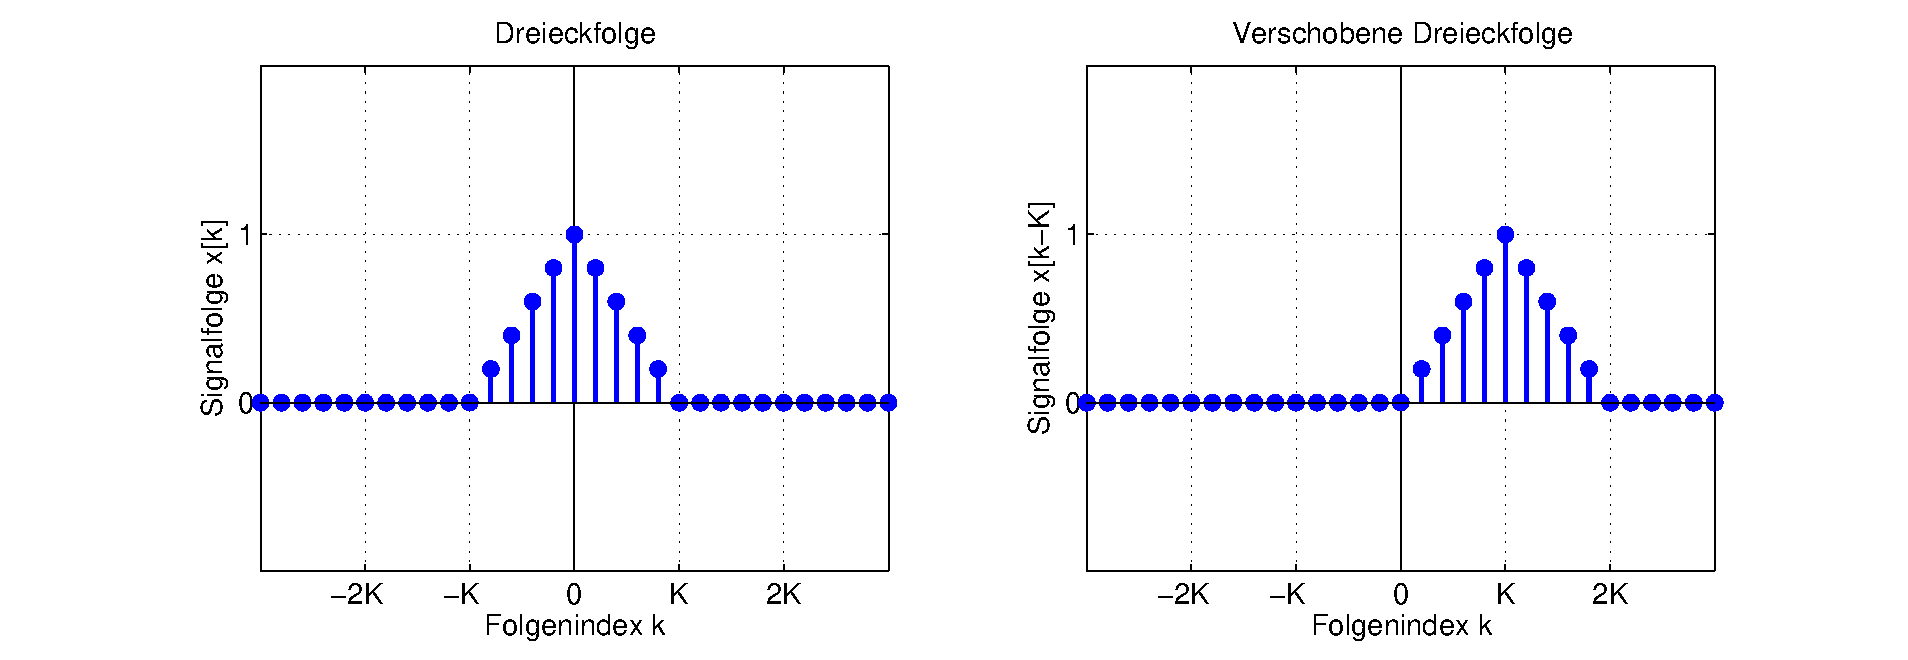
\includegraphics[width=1\textwidth]{Kapitel3/Bilder/image13.eps}}
  \caption{Dreieckfolge und verschobene Dreieckfolge}
  \label{fig:Dreieckfolge}
\end{figure}

\noindent Die Dreieckfolge ist eine Folge mit endlicher Amplitude und endlicher Dauer. Die Bedingung f\"{u}r eine Energie- und Leistungssignalfolge ist erf\"{u}llt. Wie die Rechteckfolge beginnt die Rampenfolge bereits f\"{u}r k = - K. Sie ist deshalb nicht kausal, kann aber durch Verschiebung um K nach rechts in eine kausale Folge \"{u}berf\"{u}hrt werden.

\subsubsection{Zusammenfassung Testfolgen}

\noindent In Tabelle \ref{tab:threethree} sind die wesentlichen Testfolgen und ihre Darstellungsm\"{o}glichkeiten mit der Sprungfolge zusammengefasst.

\begin{table}[H]
\setlength{\arrayrulewidth}{.1em}
\caption{Tabellarische Zusammenfassung von Testfolgen und ihrer Beschreibung mit Sprungfolgen}
\setlength{\fboxsep}{0pt}%
\colorbox{lightgray}{%
\arrayrulecolor{white}%
\begin{tabular}{| l | l |}
\hline
\parbox[c][0.45in][c]{3.3in}{\smallskip\centering\textbf{\fontfamily{phv}\selectfont{Testfolgen}}} & \parbox[c][0.45in][c]{3.3in}{\smallskip\centering\textbf{\fontfamily{phv}\selectfont{Mathematische Beschreibung durch Sprungfolgen}}}\\ \hline
\parbox[c][0.64in][c]{3.3in}{\centering{\fontfamily{phv}\selectfont{Impulsfolge}}} & 
\parbox[c][0.64in][c]{3.3in}{\centering{$\delta \left[k\right]=\sigma \left[k\right]-\sigma \left[k-1\right]$ }}\\ \hline 

\parbox[c][0.64in][c]{3.3in}{\centering{\fontfamily{phv}\selectfont{Sprungfolge}}} & 
\parbox[c][0.64in][c]{3.3in}{\centering{$\sigma \left[k\right]=\sum _{\kappa =-\infty }^{k}\delta \left[\kappa \right] $}}\\ \hline


\parbox[c][0.64in][c]{3.3in}{\centering{\fontfamily{phv}\selectfont{Rechteckfolge der L\"{a}nge 2$\cdot$K + 1}}} & \parbox[c][0.64in][c]{3.3in}{\centering{$x\left[k\right]=\sigma \left[k+K\right]-\sigma \left[k-K-1\right]$}}\\ \hline

\parbox[c][0.64in][c]{3.3in}{\centering{\fontfamily{phv}\selectfont{Signum-Folge}}} & \parbox[c][0.64in][c]{3.3in}{\centering{$x\left[k\right]=sgn\left[k\right]=2\cdot \sigma \left[k\right]-1$}}\\ \hline

\parbox[c][0.64in][c]{3.3in}{\centering\fontfamily{phv}\selectfont{{Rampenfolge}}} & 
\parbox[c][0.64in][c]{3.3in}{\centering{$x\left[k\right]=k\cdot \sigma \left[k\right]=\sum _{\kappa =-\infty }^{k}\sigma \left[\kappa -1\right] $}}\\ \hline

\end{tabular}%
}
\label{tab:threethree}
\end{table}

\clearpage

\subsection{Rechnen mit Folgen}

\noindent Die Berechnung der Ausgangsfolge eines linearen Systems kann auf bekannte Ausgangsfolgen zur\"{u}ckgef\"{u}hrt werden, wenn die Eingangsfolge auf bekannten Folgen basiert. Dazu ist es notwendig, die Folgen mit Hilfe der in diesem Abschnitt dargestellten Rechenmethoden umrechnen zu k\"{o}nnen. 

\subsubsection{Operationen mit Folgen}

\noindent F\"{u}r die Umrechnung von Folgen sind mathematische Operationen notwendig. Die wichtigsten elementaren Operationen sind im Folgenden zusammengefasst und an dem Beispiel der Folge 

\begin{equation}\label{eq:threefourtytwo}
x\left[k\right]=10\cdot r^{k} \cdot \sin \left(\Omega _{0} \cdot k\right)
\end{equation}

\noindent grafisch dargestellt.\bigskip

{\fontfamily{phv}\selectfont
\noindent\textbf{Skalierung der Amplitude}} \smallskip

\noindent Die Folge a$\cdot$x[k] ist gegen\"{u}ber der Folge x[k] verst\"{a}rkt (a $\mathrm{>}$ 1) beziehungsweise ged\"{a}mpft (0 $\mathrm{<}$ a $\mathrm{<}$ 1). Bild \ref{fig:ZeitlicheSkalierungFolgen} zeigt die Folge x[k] und die um einen Faktor 0.5 ged\"{a}mpfte Signalfolge 0.5$\cdot$x[k].

\begin{figure}[H]
  \centerline{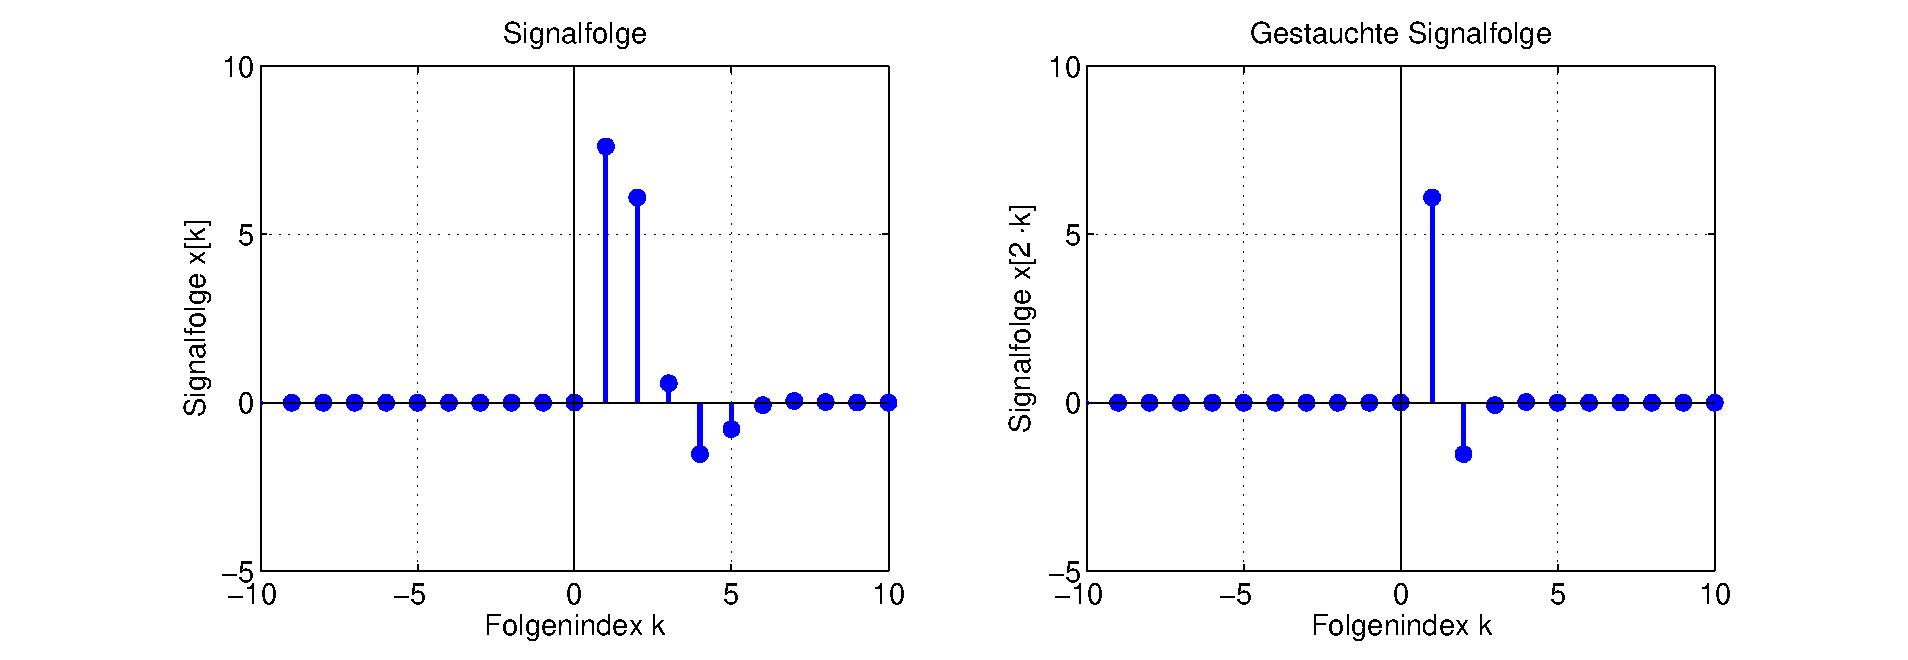
\includegraphics[width=1\textwidth]{Kapitel3/Bilder/image14.eps}}
  \caption{Darstellung der Folge x[k] und der skalierten Folge 0.5$\cdot$x[k]}
  \label{fig:ZeitlicheSkalierungFolgen}
\end{figure}

{\fontfamily{phv}\selectfont
\noindent\textbf{Zeitliche Verschiebung}} \smallskip

\noindent Die Folge $x[k - k{}_{0}]$ ist gegen\"{u}ber der Folge x[k] nach rechts $(k{}_{0} \mathrm{>} 0)$ beziehungsweise nach links $(k{}_{0} \mathrm{<} 0)$ verschoben. Bild \ref{fig:VerschibungFolgen} zeigt die Folge $x[k]$ und die um $k{}_{0} = 5$ verschobene Folge $x[k -- 5]$.

\begin{figure}[H]
  \centerline{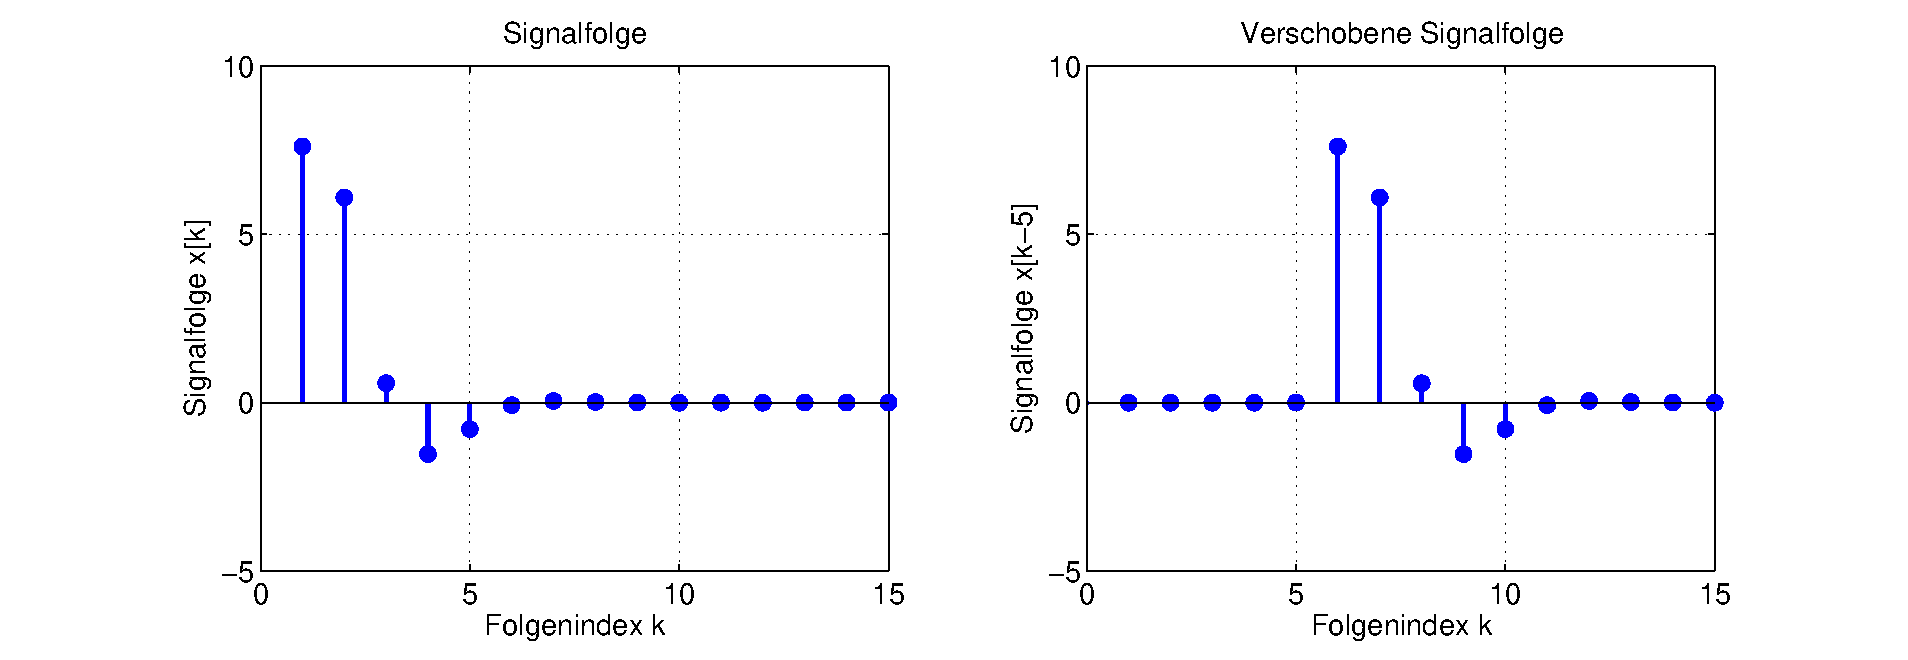
\includegraphics[width=1\textwidth]{Kapitel3/Bilder/image15.eps}}
  \caption{Darstellung der Folge x[k] und der um k${}_{0}$ = 5 nach rechts verschobenen Folge x[k -- 5]}
  \label{fig:VerschibungFolgen}
\end{figure}

\noindent Das Vorgehen wird am einfachsten deutlich, wenn \"{u}ber den Folgenindex k argumentiert wird. Die Folge x[k] weist zum Zeitpunkt k = 1 den maximalen Wert auf. Da der Index k in der Folge x[k -- 5] um 5 verringert wird, weist die Folge x[k -- 5] erst an der Stelle k = 6 den maximalen Wert auf.\bigskip

{\fontfamily{phv}\selectfont
\noindent\textbf{Spiegelung}} \smallskip

\noindent Die Spiegelung einer Folge an der Stelle k = 0 kann mathematisch durch die Folge x[-k] dargestellt werden. Bild \ref{fig:SpiegelungFolgen} zeigt die Folge x[k] und die gespiegelte Folge x[-k].

\begin{figure}[H]
  \centerline{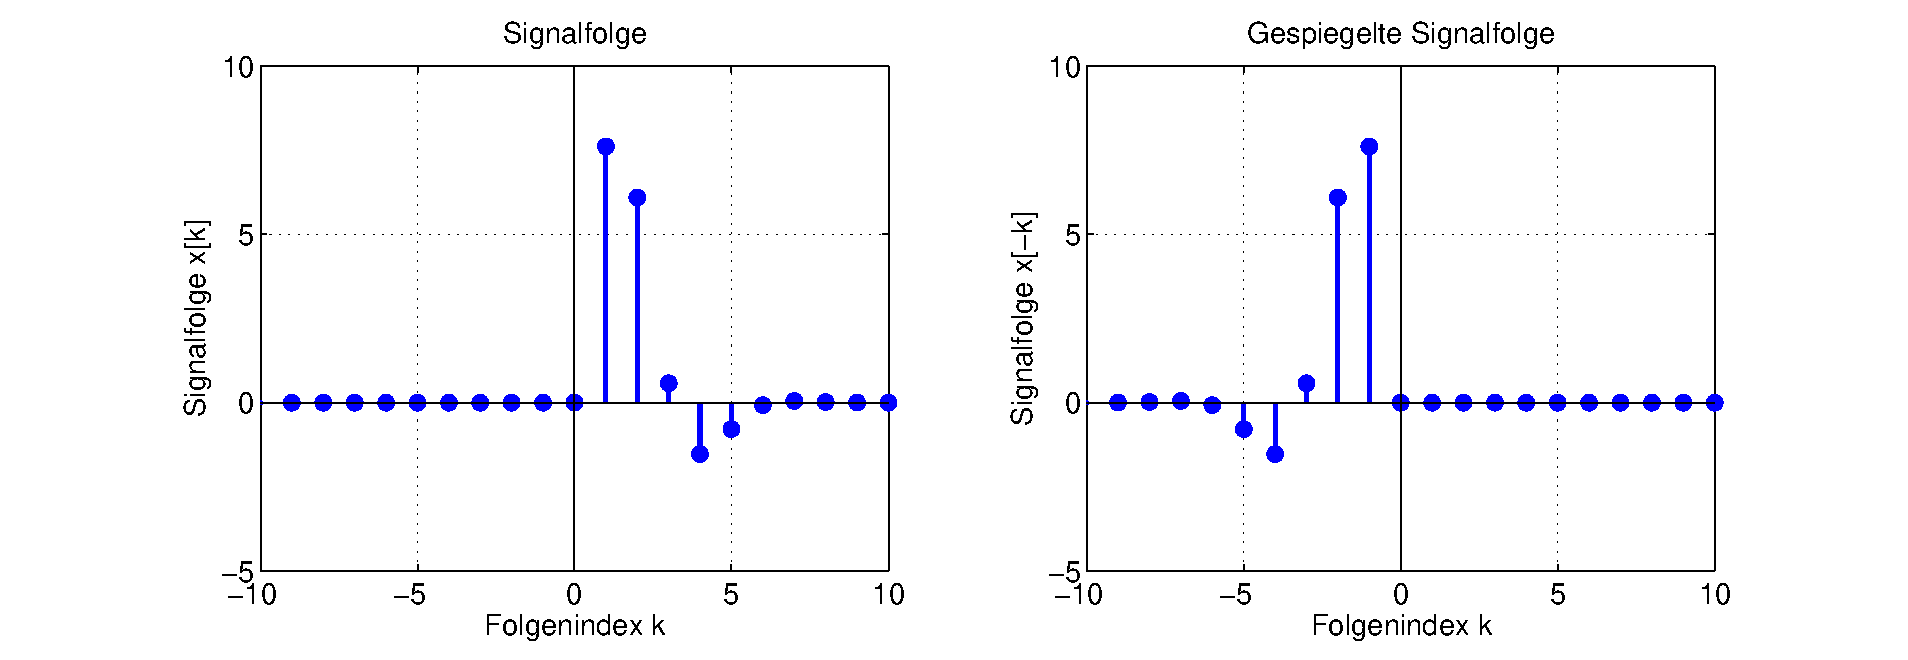
\includegraphics[width=1\textwidth]{Kapitel3/Bilder/image16.eps}}
  \caption{Darstellung der Folge x[k] und der an k = 0 gespiegelte Folge x[- k]}
  \label{fig:SpiegelungFolgen}
\end{figure}

\noindent Auch hier kann \"{u}ber den Folgenindex argumentiert werden. Die Folge x[k] weist an der Stelle k = 1 den Folgenwert x[1] = 7.6 auf. Die Folge x[-k] besitzt denselben Folgenwert an der Stelle k = - 1. \bigskip

{\fontfamily{phv}\selectfont
\noindent\textbf{Zeitliche Skalierung}} \smallskip

\noindent Bei Signalfolgen kann eine Stauchung oder Dehnung des Signals nicht beliebig vorgenommen werden, da die dazu notwenigen Abtastwerte nicht vorliegen. Ohne zus\"{a}tzliche Interpolationsschritte ist es bei der zeitlichen Skalierung nur m\"{o}glich, ganzzahlige Faktoren $a \mathrm{>} 1$ einzusetzen. Diese Skalierung f\"{u}hrt zu einer Stauchung der Signalfolge. Bild \ref{fig:StauchungFolgen} zeigt die Folge x[k] und die zeitlich skalierte Folge x[2$\cdot$k].

\begin{figure}[H]
  \centerline{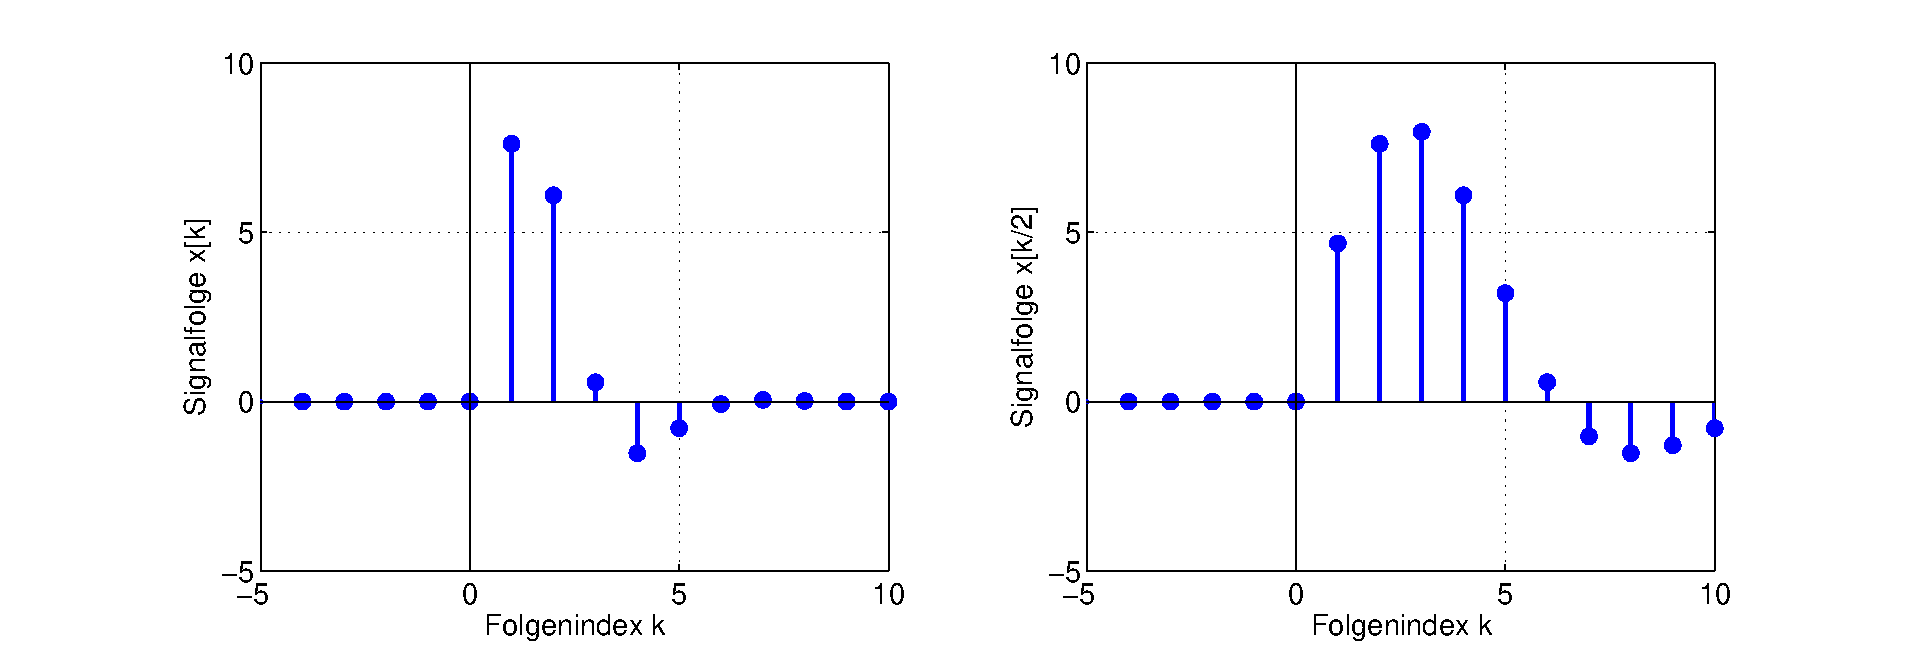
\includegraphics[width=1\textwidth]{Kapitel3/Bilder/image17.eps}}
  \caption{Darstellung der Folge x[k] und der gestauchten Signalfolge x[2$\cdot$k]}
  \label{fig:StauchungFolgen}
\end{figure}

\noindent Wieder wird der Begriff der Stauchung am einfachsten deutlich, wenn \"{u}ber das Argument der Folge $x[a\cdot k]$ argumentiert wird.

\subsubsection{\"{U}berlagerung grundlegender Folgen}

\noindent Die vorgestellten Folgen und Rechenregeln erm\"{o}glichen die Synthese weiterer Testfolgen durch eine \"{U}berlagerung grundlegender Folgen. An einem Beispiel wird das Rechnen mit grundlegenden Folgen verdeutlicht. Die Signalfolge aus Bild \ref{fig:UeberlagerungFolgen} soll als Kombination grundlegender Folgen dargestellt werden.

\begin{figure}[H]
  \centerline{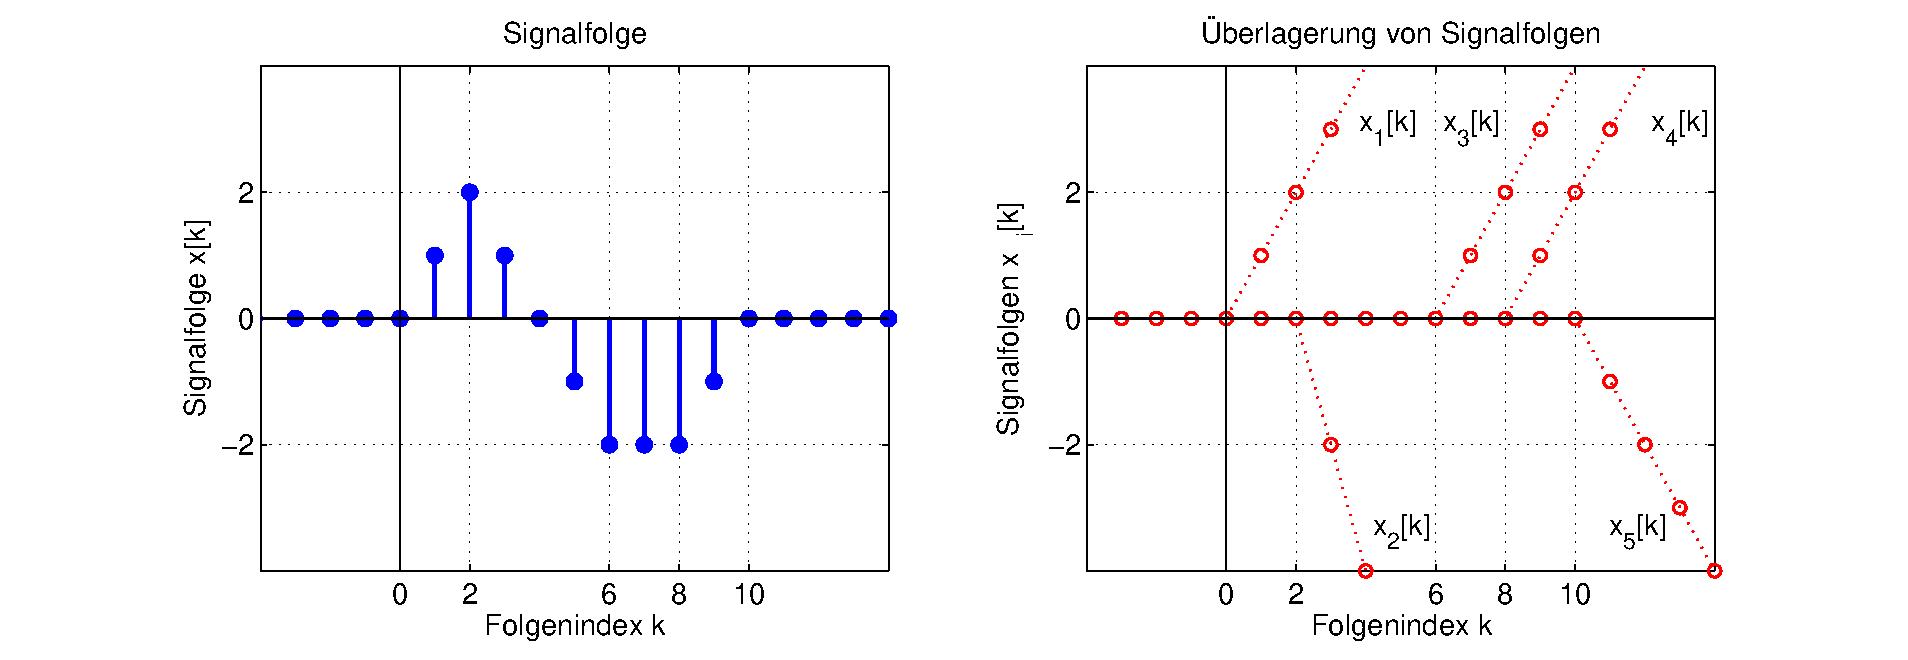
\includegraphics[width=1\textwidth]{Kapitel3/Bilder/image18.eps}}
  \caption{Darstellung einer Folge x[k] als Summe grundlegender Folgen}
  \label{fig:UeberlagerungFolgen}
\end{figure}

\noindent Bei der Beschreibung der Folge x[k] sind insbesondere die Stellen von Bedeutung, an denen sich die Steigung der Folge \"{a}ndert. Aus \ref{fig:UeberlagerungFolgen} kann abgelesen werden, dass das die Stellen 0, 2, 6, 8 und 10 sind.

\noindent An der Stelle k = 0 beginnt die Folge mit der Steigung 1. Die Folge x${}_{1}$[k], die dieses Verhalten beschreibt, lautet:

\begin{equation}\label{eq:threefourtythree}
x_{1} \left[k\right]=k\cdot \sigma \left[k\right]
\end{equation}

\noindent An der Stelle k = 2 \"{a}ndert sich die Steigung der Folge um -- 2. Der Faktor 2 ergibt sich dabei aus der Kompensation der vor dieser Stelle vorhandenen Steigung 1 und der nach der Stelle gew\"{u}nschten Steigung -- 1. Zu der Folge x${}_{1}$[k] muss die Folge x${}_{2}$[k] addiert werden, die aber erst an der Stelle k = 2 einen Einfluss haben darf. Um die Folge f\"{u}r k $\mathrm{<}$ 2 auszublenden, wird die Sprungfolge verwendet. 

\begin{equation}\label{eq:threefourtyfour}
x_{2} \left[k\right]=-2\cdot \left(k-2\right)\cdot \sigma \left[k-2\right]
\end{equation}

\noindent Das Vorgehen wiederholt sich mit unterschiedlichen Steigungs\"{a}nderungen an den Stellen 6, 8 und 10, und es ergeben sich die Folgen 

\begin{equation}\label{eq:threefourtyfive}
x_{3} \left[k\right]=\left(k-6\right)\cdot \sigma \left[k-6\right]
\end{equation}

\begin{equation}\label{eq:threefourtysix}
x_{4} \left[k\right]=\left(k-8\right)\cdot \sigma \left[k-8\right]
\end{equation}

\begin{equation}\label{eq:threefourtyseven}
x_{5} \left[k\right]=-\left(k-10\right)\cdot \sigma \left[k-10\right]
\end{equation}

\noindent Die Folge x[k] kann damit als \"{U}berlagerung der Teilfolgen x${}_{1}$[k] bis x${}_{5}$[k] dargestellt werden.

\begin{equation}\label{eq:threefourtyeight}
\begin{split}
x\left[k\right] & = k\cdot \sigma \left[k\right]-2\cdot \left(k-2\right)\cdot \sigma \left[k-2\right]+\left(k-6\right)\cdot \sigma \left[k-6\right] \\ 
& +\left(k-8\right)\cdot \sigma \left[k-8\right]-\left(k-10\right)\cdot \sigma \left[k-10\right]
\end{split}
\end{equation}

\noindent Durch den Einsatz der Sprungfolgen ist gew\"{a}hrleistet, dass die jeweilige Folge erst ab einem definierten Zeitpunkt ber\"{u}cksichtigt wird. Sie erm\"{o}glicht damit die sequenzielle Synthese der Folge x[k].

\subsubsection{Zusammenfassung Rechenoperationen mit Folgen}

\noindent In Tabelle \ref{tab:threefour} sind die besprochenen Rechenregeln zusammengefasst. Sie erm\"{o}glichen die Zerlegung von Signalfolgen in bekannte Signalanteile. Das Rechnen mit Folgen ist deshalb Grundlage f\"{u}r eine erfolgreiche Anwendung von Korrespondenztafeln der z- und Fourier-Transformation, die in Kapitel 1 und 1 beschrieben wird.

\begin{table}[H]
\setlength{\arrayrulewidth}{.1em}
\caption{Tabellarische Zusammenfassung der Rechenoperationen f\"{u}r Folgen}
\setlength{\fboxsep}{0pt}%
\colorbox{lightgray}{%
\arrayrulecolor{white}%
\begin{tabular}{| l | l |}
\hline
\parbox[c][0.35in][c]{3.3in}{\smallskip\centering\textbf{\fontfamily{phv}\selectfont{Operation}}} & \parbox[c][0.35in][c]{3.3in}{\smallskip\centering\textbf{\fontfamily{phv}\selectfont{Mathematische Beschreibung}}}\\ \hline
\parbox[c][0.64in][c]{3.3in}{\centering{\fontfamily{phv}\selectfont{Skalierung der Amplitude}}} & 
\parbox[c][0.64in][c]{3.3in}{\centering{$y\left[k\right]=a\cdot x\left[k\right]$}}\\ \hline 

\parbox[c][0.64in][c]{3.3in}{\centering{\fontfamily{phv}\selectfont{Verschiebung um k${}_{0}$ nach rechts}}} & 
\parbox[c][0.64in][c]{3.3in}{\centering{$y\left[k\right]=x\left[k-k_{0} \right]$}}\\ \hline


\parbox[c][0.64in][c]{3.3in}{\centering{\fontfamily{phv}\selectfont{Stauchung ($a \mathrm{>} 1$ und ganzzahlig)}}} & \parbox[c][0.64in][c]{3.3in}{\centering{$y\left[k\right]=x\left[a\cdot k\right]$}}\\ \hline

\parbox[c][0.64in][c]{3.3in}{\centering{\fontfamily{phv}\selectfont{Spiegelung}}} & \parbox[c][0.64in][c]{3.3in}{\centering{$y\left[k\right]=x\left[-k\right]$}}\\ \hline

\parbox[c][0.64in][c]{3.3in}{\centering{\fontfamily{phv}\selectfont{Aktivieren an der Stelle $k{}_{0}$}}} & 
\parbox[c][0.64in][c]{3.3in}{\centering{$y\left[k\right]=x\left[k\right]\cdot \sigma \left[k-k_{0} \right]$}}\\ \hline

\end{tabular}%
}
\label{tab:threefour}
\end{table}

\InsertBoxL{0}{
\includegraphics[scale=0.5]{Code.JPG}} 
\textcolor{white}{.}\newline
\noindent Im Online-Portal \textit{Systemtheorie Online} verdeutlicht die \textit{Applikation Signalabtastung und Signal-rekonstruktion} grafisch, welche Effekte durch Anti-Aliasing-Filter, reale Abtastung und reale Rekon-struktion entstehen.\newline    

\clearpage

\subsection{Folgen zur Beschreibung von zeitdiskreten Einschwingvorg\"{a}ngen}

\noindent Ausgangssignale zeitdiskreter Systeme lassen sich vielfach mit Hilfe von harmonischen Folgen und Exponentialfolgen beschreiben. Sie werden im Folgenden vorgestellt.

\subsubsection{Periodische und harmonische Folgen}

\noindent Periodische Folgen sind dadurch gekennzeichnet, dass sich der Folgenwert periodisch nach einem Intervall der L\"{a}nge K wiederholt. Bild \ref{fig:PeriodischFolge} zeigt eine einfache periodische Signalfolge:

\begin{figure}[H]
  \centerline{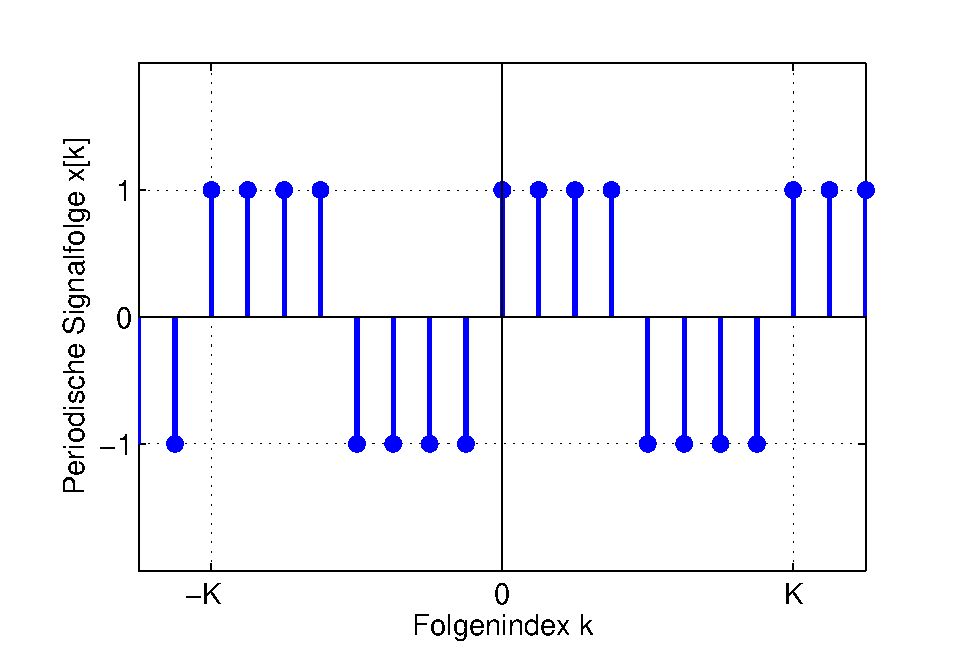
\includegraphics[width=0.5\textwidth]{Kapitel3/Bilder/image19.eps}}
  \caption{Beispiel f\"{u}r eine periodische Signalfolge mit einer Periode K = 8}
  \label{fig:PeriodischFolge}
\end{figure}

\noindent F\"{u}r periodische Folgen und ganzzahlige Werte n gilt:

\begin{equation}\label{eq:threefourtynine}
x\left[k\right]=x\left[k+n\cdot K\right]
\end{equation}

\noindent Neben den Folgen, die das Ein-, Aus- oder Umschalten modellieren, sind in der Systemtheorie periodische, harmonische Signalfolgen von gro{\ss}er Bedeutung. Als Beispiel soll hier eine Kosinusfolge diskutiert werden. Sie ist definiert als

\begin{equation}\label{eq:threefifty}
x\left[k\right]=A\cdot \cos \left(\Omega _{0} \cdot k+\varphi \right)=A\cdot \cos \left(\Omega _{0} \cdot \left(k+k_{0} \right)\right)
\end{equation}

\noindent wobei A die Amplitude der Schwingung, $\varphi$ der Nullphasenwinkel und $\Omega{}_{0}$ die normierte Kreisfrequenz ist. Die Normierung wird in Kapitel 7.1.2 ausf\"{u}hrlich diskutiert. Die normierte Kreisfrequenz ergibt sich aus dem Ansatz, dass die Folgenwerte x[k] an den Zeitpunkten k$\cdot$T${}_{A}$ mit der Funktion x(t) \"{u}bereinstimmen sollen.

\begin{equation}\label{eq:threefiftyone}
x\left[k\right]=A\cdot \cos \left(\Omega _{0} \cdot k+\varphi \right)=A\cdot \cos \left(\omega _{0} \cdot k\cdot T_{A} +\varphi \right)=x\left(k\cdot T_{A} \right)
\end{equation}

\noindent Ein Vergleich der beiden Kosinusfunktionen f\"{u}hrt zu einer Normierung der Kreisfrequenz mit der Abtastzeit T${}_{A}$. 

\begin{equation}\label{eq:threefiftytwo}
\Omega _{0} =\omega _{0} \cdot T_{A} 
\end{equation}

\noindent Da der Folgenindex k im Gegensatz zu Zeit t dimensionslos ist, besitzt die normierte Kreisfrequenz die Einheit rad. Bild \ref{fig:KosinusFolge} verdeutlicht diese Definitionen an einem Beispiel:

\begin{figure}[H]
  \centerline{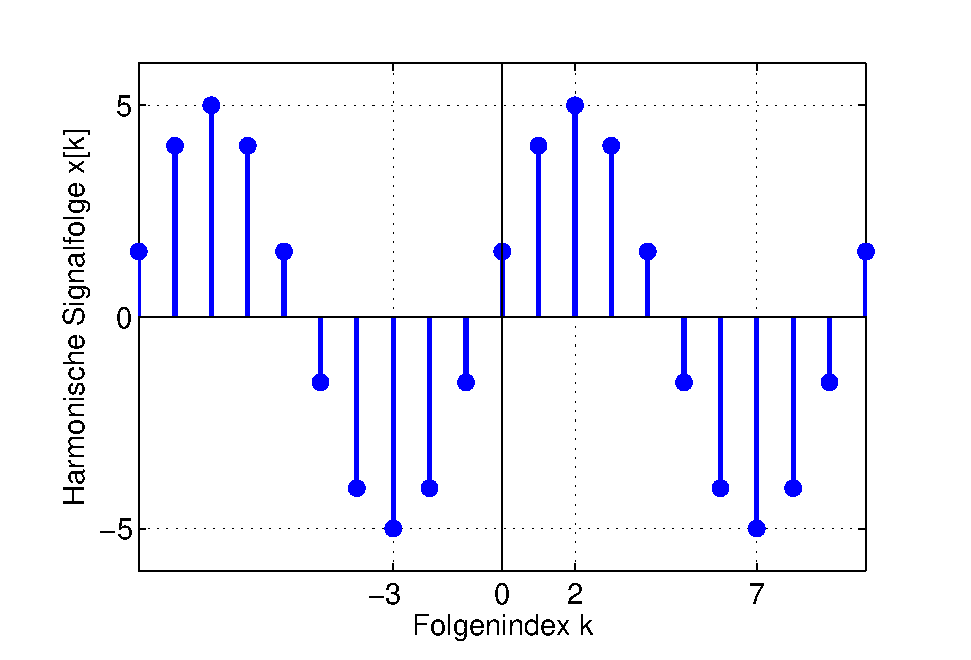
\includegraphics[width=0.5\textwidth]{Kapitel3/Bilder/image20.eps}}
  \caption{Kosinusfolge mit einer Periode K = 10, einer Amplitude von 5 und einem Nullphasenwinkel von - 2/5$\cdot\pi$}
  \label{fig:KosinusFolge}
\end{figure}

\noindent In dem Beispiel betr\"{a}gt die Amplitude 5. Die Kosinusfolge hat zwei aufeinanderfolgende Minima bei k = - 3 und k = 7, woraus sich eine Periode von K = 10 und eine normierte Kreisfrequenz 

\begin{equation}\label{eq:threefiftythree}
\Omega _{0} =\frac{2\cdot \pi }{10} 
\end{equation}

\noindent ergibt. Die Nullphase $\varphi$ ist nicht unmittelbar aus dem Diagramm ablesbar. Sie wird \"{u}ber die Verschiebung k${}_{0}$ berechnet:

\begin{equation}\label{eq:threefiftyfour}
k_{0} =\frac{\varphi }{2\cdot \pi } \cdot 10=-2
\end{equation}

\noindent F\"{u}r das Beispiel ergibt sich damit der Nullphasenwinkel $\varphi$ = - 2/5$\cdot\pi$.\bigskip

{\fontfamily{phv}\selectfont
\noindent\textbf{Zeigerdarstellung von harmonischen Signalfolgen}} \smallskip

\noindent In der Elektrotechnik hat sich f\"{u}r die Berechnung von harmonisch angeregten Schaltungen die Zeigerdarstellung durchgesetzt. Sie beruht auf der Eulerschen Formel.

\begin{equation}\label{eq:threefiftyfive}
e^{j\cdot \varphi } =\cos (\varphi )+j\cdot \sin (\varphi )
\end{equation}

\noindent Damit kann eine Kosinusfolge der Form

\begin{equation}\label{eq:threefiftysix}
x\left[k\right]=A\cdot \cos \left(\Omega _{0} \cdot k+\varphi \right)
\end{equation}

\noindent als Realteil einer komplexen Folge

\begin{equation}\label{eq:threefiftyseven}
z\left[k\right]=A\cdot e^{j\cdot \left(\Omega _{0} \cdot k+\varphi \right)} =A\cdot e^{j\cdot \varphi } \cdot e^{j\cdot \Omega _{0} \cdot k} =A\cdot \left(\cos \left(\Omega _{0} \cdot k+\varphi \right)+j\cdot \sin \left(\Omega _{0} \cdot k+\varphi \right)\right)
\end{equation}

\noindent aufgefasst werden. Diese mathematische Darstellung kann durch einen Zeiger der L\"{a}nge A verdeutlicht werden, der in der komplexen Ebene um den Koordinatenursprung rotiert. Die Zeit f\"{u}r eine volle Umdrehung ist die Periode K. Die eigentlich interessierende Gr\"{o}{\ss}e ist die Projektion des Zeigers auf die reelle Achse, sie stellt die Folge x[k] dar. Zum Zeitpunkt k = 0 gilt

\begin{equation}\label{eq:threefiftyeight}
z\left[0\right]=A\cdot e^{j\cdot \varphi } =A\cdot \cos \left(\varphi \right)+j\cdot A\cdot \sin \left(\varphi \right)
\end{equation}

\noindent Zur Verdeutlichung zeigt Bild \ref{fig:Schwingungsfolge} die Zeigerdarstellung in der komplexen Ebene.

\begin{figure}[H]
  \centerline{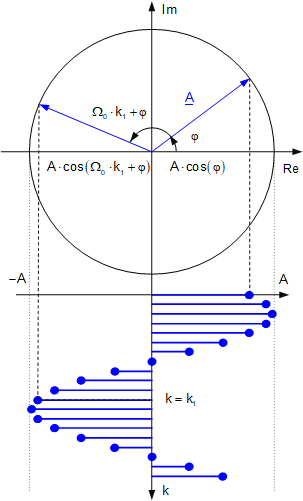
\includegraphics[width=0.55\textwidth]{Kapitel3/Bilder/image21.png}}
  \caption{Darstellung einer harmonischen Schwingungsfolge als Zeigerdiagramm}
  \label{fig:Schwingungsfolge}
\end{figure}


{\fontfamily{phv}\selectfont
\noindent\textbf{Darstellung von Signalfolgen als \"{U}berlagerung komplexer Schwingungsfolgen}} \smallskip

\noindent Durch Umformung der Eulerschen Formel ergibt sich f\"{u}r Kosinusfolgen die Darstellung

\begin{equation}\label{eq:threefiftynine}
\cos \left(\varphi \right)=\frac{1}{2} \cdot \left(e^{j\cdot \varphi } +e^{-j\cdot \varphi } \right)
\end{equation}

\noindent Damit l\"{a}sst sich die Kosinusfolge darstellen als 

\begin{equation}\label{eq:threesixty}
x\left[k\right]=A\cdot \cos \left(\Omega _{0} \cdot k+\varphi \right)=\frac{A}{2} \cdot \left(e^{j\cdot \left(\Omega _{0} \cdot k+\varphi \right)} +e^{-j\cdot \left(\Omega _{0} \cdot k+\varphi \right)} \right)
\end{equation}

\noindent Der erste Summand beschreibt einen komplexen Zeiger, der sich in der komplexen Ebene mit einer normierten Kreisfrequenz $\Omega_{0}$ in mathematisch positiver Richtung dreht. Der zweite Summand beschreibt einen zweiten komplexen Zeiger, der zu jedem Zeitpunkt konjugiert komplex zum Ersten ist. Er dreht sich mit derselben Winkelgeschwindigkeit wie der erste Zeiger, aber in entgegengesetzter Richtung. 

\clearpage

\noindent Die komplexe Exponentialfolge stellt reelle Folgen mit Hilfe komplexer Zahlen dar. Es ist eine effiziente Beschreibungsform, die gleicherma{\ss}en Amplitude und Phase beschreibt. Physikalisch gesehen existieren komplexe Signale nicht.

\InsertBoxL{0}{
\includegraphics[scale=0.5]{Code.JPG}} 
\textcolor{white}{.}\newline
\noindent Im Online-Portal \textit{Systemtheorie Online} verdeutlicht die \textit{Applikation Signalabtastung und Signal-rekonstruktion} grafisch, welche Effekte durch Anti-Aliasing-Filter, reale Abtastung und reale Rekon-struktion entstehen.\newline   

\subsubsection{Exponentialfolge}

\noindent Bei der Diskussion von zeitdiskreten Systemen wird sich zeigen, dass die Exponentialfolge 

\begin{equation}\label{eq:threesixtyone}
x\left[k\right]=A\cdot r_{0}^{k} \cdot \sigma \left[k\right]
\end{equation}

\noindent die Einschwingvorg\"{a}nge vieler linearer zeitdiskreter Systeme beschreibt. Bild \ref{fig:ExponentialFolgeunParam} stellt das Verhalten der Exponentialfolge f\"{u}r unterschiedliche reelle Parameter r${}_{0}$ und k $\mathrm{>}$ 0 dar:

\begin{figure}[H]
  \centerline{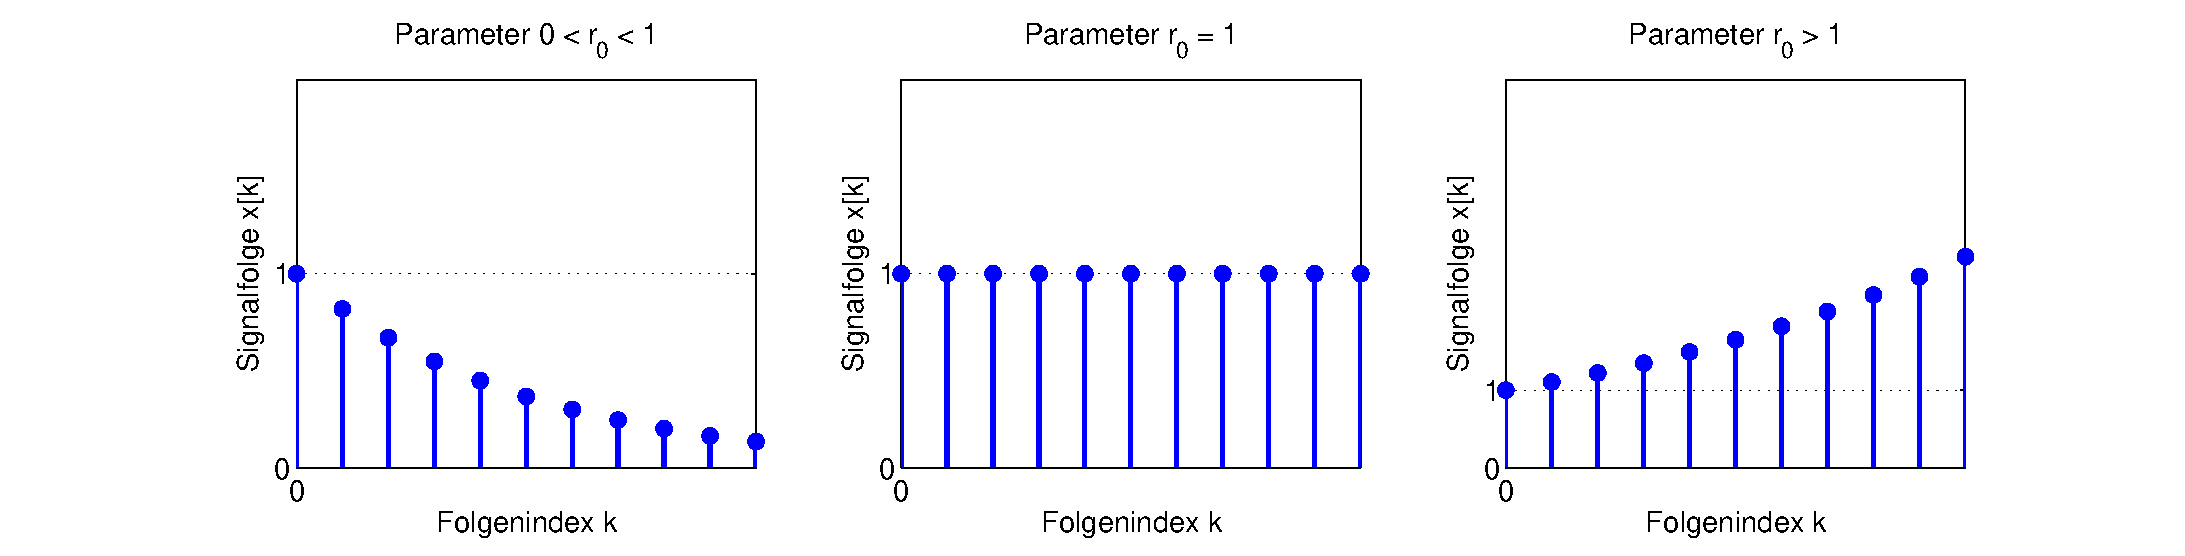
\includegraphics[width=1\textwidth]{Kapitel3/Bilder/image22.eps}}
  \caption{Darstellung der Exponentialfolge f\"{u}r unterschiedliche Parameter r${}_{0}$}
  \label{fig:ExponentialFolgeunParam}
\end{figure}

\noindent Die Exponentialfolge beginnt f\"{u}r alle Parameter r${}_{0}$ an der Stelle x[0] = A. F\"{u}r reelle Parameter 0 $\mathrm{<}$ r${}_{0}$ $\mathrm{<}$ 1 n\"{a}hert sich die Exponentialfolge der Asymptote x = 0. F\"{u}r r${}_{0}$ = 1 bleibt die Exponentialfolge konstant bei x = A. F\"{u}r r${}_{0}$ $\mathrm{>}$ 1 steigt die Exponentialfolge mit wachsendem Folgenindex k.

\noindent Mit Exponentialfolgen der Form e$^{j\Omega_{0}\cdot k}$ k\"{o}nnen harmonische Schwingungen beschrieben werden. Durch die Kombination beider Exponentialfolgen k\"{o}nnen Kosinusfolgen mit exponentiell abklingender Amplitude als Summe zweier Exponentialfolgen dargestellt werden. 

\begin{equation}\label{eq:threesixtytwo}
\begin{split}
x\left[k\right] & = A\cdot r_{0}^{k} \cdot \cos \left(\Omega _{0} \cdot k\right)\cdot \sigma \left[k\right]=\frac{1}{2} \cdot A\cdot r_{0}^{k} \cdot \left(e^{j\cdot \Omega _{0} \cdot k} +e^{-j\cdot \Omega _{0} \cdot k} \right)\cdot \sigma \left[k\right]\\ 
& = \frac{1}{2} \cdot A\cdot \left(\left(r_{0} \cdot e^{j\cdot \Omega _{0} } \right)^{k} +\left(r_{0} \cdot e^{-j\cdot \Omega _{0} } \right)^{k} \right)\cdot \sigma \left[k\right]=\frac{1}{2} \cdot A\cdot \left(\lambda _{0}^{k} +\left(\lambda _{0}^{*} \right)^{k} \right)\cdot \sigma \left[k\right]
\end{split}
\end{equation}

\noindent Die Kosinusfolge mit exponentiell abklingender Amplitude ist in Bild \ref{fig:ExponentialFolgeunabkAmp} dargestellt. Dabei sind die Einh\"{u}llenden der Kosinusfolge als gestrichelte Linie eingezeichnet.

\clearpage

\begin{figure}[H]
  \centerline{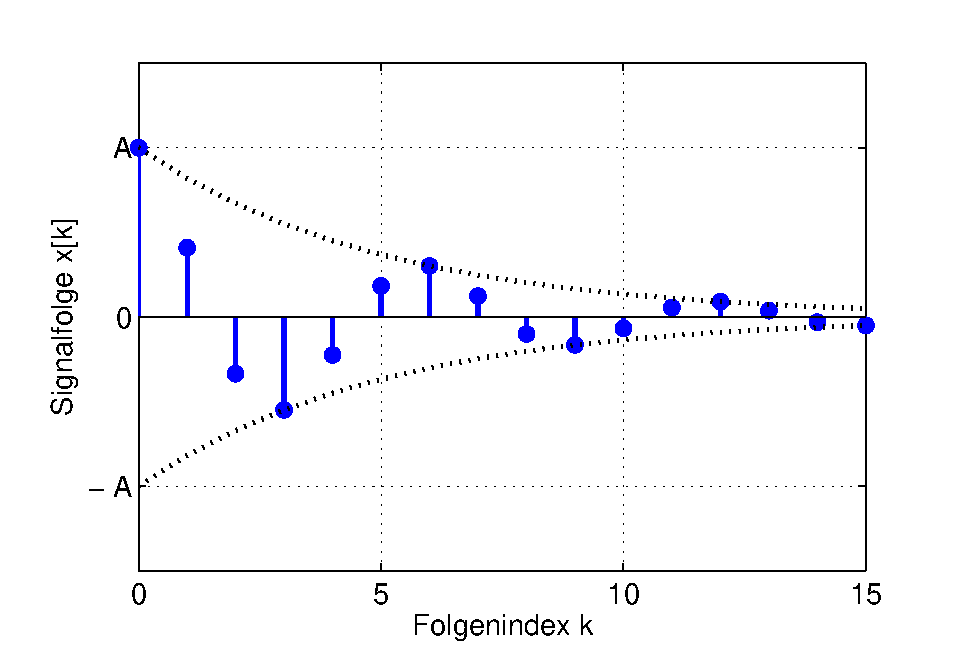
\includegraphics[width=0.5\textwidth]{Kapitel3/Bilder/image23.eps}}
  \caption{Darstellung einer Exponentialfolge mit abklingender Amplitude}
  \label{fig:ExponentialFolgeunabkAmp}
\end{figure}

\noindent Je nach Lage des Wertes $\lambda_{0}$ = r$_{0} \cdot$ e$^{j\Omega_{0}\cdot k}$ in der komplexen Ebene ergeben sich ein charakteristisches Verhalten der komplexen Exponentialfolge. Bei der Diskussion von Systemeigenschaften linearer Systeme wird die Interpretation reeller und komplexer Exponentialfolgen weiter vertieft.

\InsertBoxL{0}{
\includegraphics[scale=0.5]{Code.JPG}} 
\textcolor{white}{.}\newline
\noindent Im Online-Portal \textit{Systemtheorie Online} verdeutlicht die \textit{Applikation Signalabtastung und Signal-rekonstruktion} grafisch, welche Effekte durch Anti-Aliasing-Filter, reale Abtastung und reale Rekon-struktion entstehen.\newline   

\clearpage

\subsubsection{Zusammenfassung zur Beschreibung von zeitdiskreten Einschwingvorgängen}

\noindent Die Systemreaktion linearer zeitdiskreter Systeme ist in vielen Anwendungen eine abklingende harmonische Schwingungsfolge. Zur mathematischen Beschreibung werden in Tabelle \ref{tab:threefive} Folgen zusammengestellt.

\begin{table}[H]
\setlength{\arrayrulewidth}{.1em}
\caption{Folgen zur Beschreibung von Einschwingvorgängen}
\setlength{\fboxsep}{0pt}%
\colorbox{lightgray}{%
\arrayrulecolor{white}%
\begin{tabular}{| c | c |}
\hline
\parbox[c][0.35in][c]{3.3in}{\smallskip\centering\textbf{\fontfamily{phv}\selectfont{Folge}}} & \parbox[c][0.35in][c]{3.3in}{\smallskip\centering\textbf{\fontfamily{phv}\selectfont{Mathematische Beschreibung}}}\\ \hline
\parbox[c][0.64in][c]{3.3in}{\centering{\fontfamily{phv}\selectfont{Periodische Folge der Periodendauer K}}} & 
\parbox[c][0.64in][c]{3.3in}{\centering{$x\left[k\right]=x\left[k+n\cdot K\right]$}}\\ \hline 

\parbox[c][0.64in][c]{3.3in}{\centering{\fontfamily{phv}\selectfont{Harmonische Folge}}} & 
\parbox[c][0.64in][c]{3.3in}{\centering{$x\left[k\right]=A\cdot \cos \left(\Omega _{0} \cdot k+\varphi \right)=A\cdot \cos \left(\Omega _{0} \cdot \left(k+k_{0} \right)\right)$}}\\ \hline


\parbox[c][0.64in][c]{3.3in}{\centering{\fontfamily{phv}\selectfont{Eulersche Formel}}} & 
\parbox[c][0.64in][c]{3.3in}{\centering{$e^{j\cdot \varphi } =\cos \left(\varphi \right)+j\cdot \sin \left(\varphi \right)$}}\\ \hline

\parbox[c][0.64in][c]{3.3in}{\centering{\fontfamily{phv}\selectfont{Darstellung der Kosinusfolge über\\
die Eulersche Formel}}} & 
\parbox[c][0.64in][c]{3.3in}{\centering{$\cos \left(\Omega _{0} \cdot k\right)=\frac{1}{2} \cdot \left(e^{j\cdot \Omega _{0} \cdot k} +e^{-j\cdot \Omega _{0} \cdot k} \right)$}}\\ \hline

\parbox[c][0.64in][c]{3.3in}{\centering{\fontfamily{phv}\selectfont{Darstellung der Sinusfolge über\\
die Eulersche Formel}}} & 
\parbox[c][0.64in][c]{3.3in}{\centering{$\sin \left(\Omega _{0} \cdot k\right)=\frac{1}{2\cdot j} \cdot \left(e^{j\cdot \Omega _{0} \cdot k} -e^{-j\cdot \Omega _{0} \cdot k} \right)$}}\\ \hline

\parbox[c][0.64in][c]{3.3in}{\centering{\fontfamily{phv}\selectfont{Exponentialfolge mit komplexem Argument}}} & 
\parbox[c][0.64in][c]{3.3in}{\centering{$\lambda _{0}^{k} =\left(r_{0} \cdot e^{j\cdot \Omega _{0} } \right)^{k} =r_{0}^{k} \cdot e^{j\cdot \Omega _{0} \cdot k} $}}\\ \hline

\parbox[c][1in][c]{3.3in}{\centering{\fontfamily{phv}\selectfont{Beschreibung einer gedämpften Schwingungsfolge
über eine Exponentialfolge mit komplexem Argument}}} & 
\parbox[c][1in][c]{3.3in}{\centering{$\begin{array}{rcl} {x\left[k\right]} & {=} & {A\cdot r_{0}^{k} \cdot \cos \left(\Omega _{0} \cdot k\right)\cdot \sigma \left[k\right]} \\ {} & {=} & {\frac{1}{2} \cdot A\cdot \left(\left(r_{0} \cdot e^{j\cdot \Omega _{0} } \right)^{k} +\left(r_{0} \cdot e^{-j\cdot \Omega _{0} } \right)^{k} \right)\cdot \sigma \left[k\right]} \\ {} & {=} & {\frac{1}{2} \cdot A\cdot \left(\lambda ^{k} +\lambda ^{*} {}^{k} \right)\cdot \sigma \left[k\right]} \end{array}$ }}\\ \hline

\end{tabular}%
}
\label{tab:threefive}
\end{table}

\clearpage

\subsection{Literatur}

\subsubsection{Literaturstellen mit besonders anschaulicher Darstellung}

\begin{tabular}{|p{0.7in}|p{5in}|} \hline 
[Lyon04] & Lyons, Richard G.: Understanding Digital Signal Processing, \newline Prentice Hall, New Jersey, 2004 \\ \hline 
[Stea99] & Stearns, Samuel: Digitale Verarbeitung analoger Signale, \newline 7. Auflage, Oldenbourg Verlag M\"{u}nchen, 1999 \\ \hline 
\end{tabular}


\subsubsection{Literaturstellen mit praktischen Anwendungen}

\begin{tabular}{|p{0.7in}|p{5.5in}|} \hline 
[Wern08] & Werner, Martin: Signale und Systeme,\newline Vieweg Studium Technik, Wiesbaden, 2008 \\ \hline 
[Meye08] & Meyer, Martin: Signalverarbeitung -- Analoge und digitale Signal, Systeme und Filter,\newline Vieweg Studium Technik, Wiesbaden, 2008 \\ \hline 
\end{tabular}


\subsubsection{Weiterf\"{u}hrende Literatur}

\begin{tabular}{|p{0.7in}|p{5in}|} \hline 
[Oppe04] & Oppenheim, Alan: Zeitdiskrete Signalverarbeitung,2.\newline \"{u}berarbeitete Auflage, Pearson Studium, 2004 \\ \hline 
[Kamm98] & Kammeyer, Karl: Digitale Signalverarbeitung, \newline B.G. Teubner Stuttgart, 1998 \\ \hline 
\end{tabular}